%%%%%%%%%%%%%%%%%%%%%%%%%%%%%%%%%%%%%%%%%
% Wenneker Article
% LaTeX Template
% Version 2.0 (28/2/17)
%
% This template was downloaded from:
% http://www.LaTeXTemplates.com
%
% Authors:
% Vel (vel@LaTeXTemplates.com)
% Frits Wenneker
%
% License:
% CC BY-NC-SA 3.0 (http://creativecommons.org/licenses/by-nc-sa/3.0/)
%
%%%%%%%%%%%%%%%%%%%%%%%%%%%%%%%%%%%%%%%%%

%----------------------------------------------------------------------------------------
%	PACKAGES AND OTHER DOCUMENT CONFIGURATIONS
%----------------------------------------------------------------------------------------

\documentclass[11pt, a4paper]{article} % 10pt font size (11 and 12 also possible), A4 paper (letterpaper for US letter) and two column layout (remove for one column)

\usepackage[english]{babel} % English language hyphenation
\usepackage{microtype} % Better typography
\usepackage{amsmath,amsfonts,amsthm} % Math packages for equations
\usepackage[svgnames]{xcolor,colortbl} % Enabling colors by their 'svgnames'
\usepackage[hang, small, labelfont=bf, up, textfont=it]{caption} % Custom captions under/above tables and figures
\usepackage{booktabs} % Horizontal rules in tables
\usepackage{lastpage} % Used to determine the number of pages in the document (for "Page X of Total")
\usepackage{graphicx} % Required for adding images
\usepackage{amssymb}
\usepackage[mathscr]{eucal}
\usepackage[table]{xcolor}
\usepackage{enumitem} % Required for customising lists
\setlist{noitemsep} % Remove spacing between bullet/numbered list elements
\usepackage{sectsty} % Enables custom section titles
\allsectionsfont{\usefont{OT1}{phv}{b}{n}} % Change the font of all section commands (Helvetica)
\usepackage{hyperref}
\usepackage[sort,numbers]{natbib}
\usepackage{fancyhdr}
\usepackage{url}
\usepackage{floatrow}
\usepackage{sidecap}
\usepackage{hyperref}

\definecolor{Gray}{gray}{0.85}
\definecolor{LightCyan}{rgb}{0.88,1,1}
\definecolor{LightPink}{rgb}{0.25,0.5,1}
\definecolor{bubblegum}{rgb}{0.99, 0.76, 0.8}
\definecolor{pastelpink}{rgb}{1.0, 0.82, 0.86}
\definecolor{piggypink}{rgb}{0.99, 0.87, 0.85}
\definecolor{pink}{rgb}{1, 0.5, 0.9}
\definecolor{lightpink}{rgb}{1.0, 0.61, 0.76}

% ----------------------------------------------------------------------------------------
%	MARGINS AND SPACING
%----------------------------------------------------------------------------------------
\usepackage{geometry} % Required for adjusting page dimensions
\geometry{
	top=1.5cm, % Top margin
	bottom=1.5cm, % Bottom margin
	left=1.5cm, % Left margin
	right=1.5cm, % Right margin
	includehead, % Include space for a header
	includefoot, % Include space for a footer
	%showframe, % Uncomment to show how the type block is set on the page
}
\setlength{\columnsep}{6mm} % Column separation width

%----------------------------------------------------------------------------------------
%	FONTS
%----------------------------------------------------------------------------------------

\usepackage[T1]{fontenc} % Output font encoding for international characters
\usepackage[utf8]{inputenc} % Required for inputting international characters
\usepackage{XCharter} % Use the XCharter font
\usepackage{verbatim} 
%\usepackage{fontspec}
%\setmainfont{TeX Gyre Termes}
\pagestyle{headings}
\usepackage{fancyhdr}
\setlength{\headheight}{15.2pt}
\pagestyle{fancy}
%%%%%%%%%%%%%%%%%%%%%%%%%%%%%%%%%%%%%%%%%%
% Wenneker Article
% Structure Specification File
% Version 1.0 (28/2/17)
%
% This file originates from:
% http://www.LaTeXTemplates.com
%
% Authors:
% Frits Wenneker
% Vel (vel@LaTeXTemplates.com)
%
% License:
% CC BY-NC-SA 3.0 (http://creativecommons.org/licenses/by-nc-sa/3.0/)
%
%%%%%%%%%%%%%%%%%%%%%%%%%%%%%%%%%%%%%%%%%

%----------------------------------------------------------------------------------------
%	PACKAGES AND OTHER DOCUMENT CONFIGURATIONS
%----------------------------------------------------------------------------------------

\usepackage[english]{babel} % English language hyphenation

\usepackage{microtype} % Better typography

\usepackage{amsmath,amsfonts,amsthm} % Math packages for equations

\usepackage[svgnames]{xcolor} % Enabling colors by their 'svgnames'

\usepackage[hang, small, labelfont=bf, up, textfont=it]{caption} % Custom captions under/above tables and figures

\usepackage{booktabs} % Horizontal rules in tables

\usepackage{lastpage} % Used to determine the number of pages in the document (for "Page X of Total")

\usepackage{graphicx} % Required for adding images

\usepackage{enumitem} % Required for customising lists
\setlist{noitemsep} % Remove spacing between bullet/numbered list elements

\usepackage{sectsty} % Enables custom section titles
\allsectionsfont{\usefont{OT1}{phv}{b}{n}} % Change the font of all section commands (Helvetica)

%----------------------------------------------------------------------------------------
%	MARGINS AND SPACING
%----------------------------------------------------------------------------------------

\usepackage{geometry} % Required for adjusting page dimensions

\geometry{
	top=1cm, % Top margin
	bottom=1.5cm, % Bottom margin
	left=2cm, % Left margin
	right=2cm, % Right margin
	includehead, % Include space for a header
	includefoot, % Include space for a footer
	%showframe, % Uncomment to show how the type block is set on the page
}

\setlength{\columnsep}{7mm} % Column separation width

%----------------------------------------------------------------------------------------
%	FONTS
%----------------------------------------------------------------------------------------

\usepackage[T1]{fontenc} % Output font encoding for international characters
\usepackage[utf8]{inputenc} % Required for inputting international characters

\usepackage{XCharter} % Use the XCharter font

%----------------------------------------------------------------------------------------
%	HEADERS AND FOOTERS
%----------------------------------------------------------------------------------------

\usepackage{fancyhdr} % Needed to define custom headers/footers
\pagestyle{fancy} % Enables the custom headers/footers

\renewcommand{\headrulewidth}{0.0pt} % No header rule
\renewcommand{\footrulewidth}{0.4pt} % Thin footer rule

\renewcommand{\sectionmark}[1]{\markboth{#1}{}} % Removes the section number from the header when \leftmark is used

%\nouppercase\leftmark % Add this to one of the lines below if you want a section title in the header/footer

% Headers
\lhead{} % Left header
\chead{\textit{\thetitle}} % Center header - currently printing the article title
\rhead{} % Right header

% Footers
\lfoot{} % Left footer
\cfoot{} % Center footer
\rfoot{\footnotesize Page \thepage\ of \pageref{LastPage}} % Right footer, "Page 1 of 2"

\fancypagestyle{firstpage}{ % Page style for the first page with the title
	\fancyhf{}
	\renewcommand{\footrulewidth}{0pt} % Suppress footer rule
}

%----------------------------------------------------------------------------------------
%	TITLE SECTION
%----------------------------------------------------------------------------------------

\newcommand{\authorstyle}[1]{{\large\usefont{OT1}{phv}{b}{n}\color{DarkRed}#1}} % Authors style (Helvetica)

\newcommand{\institution}[1]{{\footnotesize\usefont{OT1}{phv}{m}{sl}\color{Black}#1}} % Institutions style (Helvetica)

\usepackage{titling} % Allows custom title configuration

\newcommand{\HorRule}{\color{DarkGoldenrod}\rule{\linewidth}{1pt}} % Defines the gold horizontal rule around the title

\pretitle{
	\vspace{-30pt} % Move the entire title section up
	\HorRule\vspace{10pt} % Horizontal rule before the title
	\fontsize{32}{36}\usefont{OT1}{phv}{b}{n}\selectfont % Helvetica
	\color{DarkRed} % Text colour for the title and author(s)
}

\posttitle{\par\vskip 15pt} % Whitespace under the title

\preauthor{} % Anything that will appear before \author is printed

\postauthor{ % Anything that will appear after \author is printed
	\vspace{10pt} % Space before the rule
	\par\HorRule % Horizontal rule after the title
	\vspace{20pt} % Space after the title section
}

%----------------------------------------------------------------------------------------
%	ABSTRACT
%----------------------------------------------------------------------------------------

\usepackage{lettrine} % Package to accentuate the first letter of the text (lettrine)
\usepackage{fix-cm}	% Fixes the height of the lettrine

\newcommand{\initial}[1]{ % Defines the command and style for the lettrine
	\lettrine[lines=3,findent=4pt,nindent=0pt]{% Lettrine takes up 3 lines, the text to the right of it is indented 4pt and further indenting of lines 2+ is stopped
		\color{DarkGoldenrod}% Lettrine colour
		{#1}% The letter
	}{}%
}

\usepackage{xstring} % Required for string manipulation

\newcommand{\lettrineabstract}[1]{
	\StrLeft{#1}{1}[\firstletter] % Capture the first letter of the abstract for the lettrine
	\initial{\firstletter}\textbf{\StrGobbleLeft{#1}{1}} % Print the abstract with the first letter as a lettrine and the rest in bold
}

%----------------------------------------------------------------------------------------
%	BIBLIOGRAPHY
%----------------------------------------------------------------------------------------

\usepackage[backend=bibtex,style=authoryear,natbib=true]{biblatex} % Use the bibtex backend with the authoryear citation style (which resembles APA)

\addbibresource{example.bib} % The filename of the bibliography

\usepackage[autostyle=true]{csquotes} % Required to generate language-dependent quotes in the bibliography
 % Specifies the document structure and loads requires packages
\fancyhf{}
%\fancyhead[LE,RO]{Overleaf}
%\fancyhead[RE,LO]{Guides and tutorials}
%\fancyfoot[LO,RE]{FETOPEN-01 template WP18-20 v20171106}
\fancyfoot[LE,RO]{$\mathcal{ROBHOOT}$}
%\fancyfoot[LE,RE]{\thepage} % pa
\fancyfoot[L]{\thepage}
%----------------------------------------------------------------------------------------
%	ARTICLE INFORMATION
%----------------------------------------------------------------------------------------
\begin{document}

%\title{$\mathcal{ROBHOOT}$ \\ Open Discovery Network \\ v.1.0}} % The article title
\title{$\mathcal{ROBHOOT}$ \\ Knowledge Discovery in Evolutionary Biology-Inspired Federated Networks \\ v.3.0}}
%Automated Discovery Knowledge Graphs in Evolving Heterogeneous Federated Networks

%The article title
  %\author{{\textsuperscript{1,2,3} and XY\textsuperscript{2,3}}% Authors
  \newline\newline % Space before institutions
  \\
%	\textsuperscript{1}\institution{}\\ % Institution 1
%	\textsuperscript{2}\institution{}\\ % Institution 2
	%\textsuperscript{3}\institution{\texttt{LaTeXTemplates.com}}
      %} % Institution 3


% Example of a one line author/institution relationship
%\author{\newauthor{John Marston} \newinstitution{Universidad Nacional Autónoma de México, Mexico City, Mexico}}

\date{\today} % Add a date here if you would like one to appear underneath the title block, use \today for the current date, leave empty for no date
%---------------------------------------------------------------------------------------

%\pagestyle{plain}
\maketitle % Print the title
%\thispagestyle{firstpage} % Apply the page style for the first page (no headers and footers)

\tableofcontents

%----------------------------------------------------------------------------------------
%	ABSTRACT
%----------------------------------------------------------------------------------------
\section*{{\bf Summary}} Global sustainability is a major goal of
humanity. Many studies have shown global sustainability could be
achieved by strengthening transparency, communication, and rapid
access to reproducible information among social, ecological,
economical, technological and governance systems. Sustainability
goals, however, strongly depend on global access to evidence-, and
discovery-based knowledge gaps. Yet, science-enabled technologies
targeting knowledge discovery to reach sustainability and biodiversity
conservation goals are not in place. We propose a evolutionary
biology- and AI-inspired knowledge discovery technology for a
sustainable-, and knowledge-inspired society. We introduce
evolutionary biology- and AI-inspired solutions to account for large and
heterogeneous groups in federated networks to explore sustainable
scenarios for the international exploration of the Seas. Knowledge
discovery running on a federated network encompass a hybrid-technology
to lay out the foundation of an open- and cooperative-science
ecosystem to automate discovery in global emergency and sustainability
challenges. The project summarized here is not set out to deliver
automated discovery knowledge in federated networks, but to provide
the architecture of a science-enabled technology, as a
proof-of-principle, to connect global human sustainability challenges
to knowledge-inspired societies.
%----------------------------------------------------------------------------------------
%	ARTICLE CONTENTS
% ----------------------------------------------------------------------------------------
\section{Excellence}
\subsection{Radical vision of a science-enabled technology}
We are in the midst of the fourth industrial revolution, a
transformation revolving around data-driven intelligent machines and
knowledge-inspired societies. More than half of the global population
is now online using the Internet (i.e., 3.9 billion), which represents
a more inclusive global information society ({\bf +++}). The Internet
is rapidly evolving and people are using technology in powerful ways,
from adopting decentralized technologies for humanitarian efforts to
improving agricultural practices and reducing waste in the global food
supply chain (\citep{Wilson2018},+++). Data analytics is advancing at
a pace dictated by the availability of data. A myriad of data-driven
approaches are being developed to extract patterns from data
(\citep{Schmidhuber:2015}). At the same time, data analytics is being
challenged because the diversity of data sources keeps rising ({\bf
  +++}). Consequntly, Artifical Intelligence (AI) approaches are
rapidly evolving towards more explainable/interpretable pattern
inference ({\bf +++}). The digital ecosystem has to deploy
science-enabled technologies that account for the increasing data
heterogeneity and interpretability. However, science-enabled
technologies accounting for these two features are scarce
\citep{RePEc}.
  
Taken together, the transformation of a digital society into a
knowledge-inspired society requires solving several gaps. First, the
science-enabled technological paradigm for assisting humans is biased
towards a limited range of the ``observable'' heterogeneity in
data-sources. Thus, it limits the number of interpretable patterns
({\bf +++}). Second, the AI technological paradigm is rooted in
single- and multiple-objective optimizations (i.e., function loss or
reward, similar to fitness optima functions in evolutionary biology
{\bf +++}). Optimization-based technologies have produced a great deal
of progress, yet, they limit a broader number of sub-optimal but
plausible solutions, as usually found in evolving biological systems
({\bf +++}). And third, science-enabled technologies for scientific
inquiries are highly fragmented, only partly reproducible, and mostly
developed in close-source software
(\citep{Inhaber1977,Ioannidis2005,Fang2011,Gunther2018,Hardwicke2018,Mehrabi2019,Real2020}). To
leverage the abundance and heterogeneity of data, a) a science-enabled
technology should be able to obtain information from a large pool of
heterogeneous data-sources, b) the analysis of the data should go
beyond the identification and interpretation of patterns, and towards
the discovery knowledge gap and to the end-user, c) the analysis
should be performed in a federate way, such that highly heterogeneous
populations can learn from each other to reach consensus about the
population of plausible scenarios accounting for data heterogeneity
and dimensionality, and d) the whole process should be automated,
reproducible and transparent such that can be improved to benefit the
public. Our project contributes towards a discovery science-enabled
technology, where novel rules and interactions are exposed to
federated networks inspired by evolutionary biology and neural biology
(Figures 1 and 2 and Table 1). Evolutionary dynamics-inspired
technologies allow studying consensus algorithms within and between
groups to enrich knowledge-inspired societies facing global
sustainability problems. They do so through extracting information
from highly heterogeneous and multidimensional groups while minimizing
the need of having optimal solutions. This is particularly relevant
when discovery is obtained from heterogeneous data-sources to gain
information of complex governance, social, environmental and
technological problems (Figure 2) \citep{Mastrangelo2019}.

% Evolutionary computation models accounting for multidimensionality
% and node heterogeneity are rare
Many experimental evolution and evolutionary computation models have
shown the plausibility of coexistence of multiple heterogeneous
populations ({\bf +++}). Many interpretable mechanisms have been
proposed to explain such a coexistence, like negative-frequency
dependent selection (Doebeli book and others, {\bf +++}),
fluctuating-selection, and many others ({\bf +++}). Yet, approaches
accounting for not optimal or maladaptive solutions in the context of
group heterogeneity in multidimensional landscapes are rare (refs
around evolution cooperation in multidimensional landscapes, {\bf
  +++}). In ecological systems, intraspecific trait variation (i.e., a
proxy for heterogeneity within a species) and trait dimensionality
(i.e., biotic, reproductive, abiotic and migration traits for example)
can drive functional interactions with other species (i.e.,
cooperative, antagonistic, competitive, or mutualistic), but most
approaches have neglected the effect of trait dimensionality like
competition and cooperation traits in heterogeneous populations {\bf
  (On neural systems, the vast majority of neurons in the brain show
  highly differentitated morphological, genetic and phenotypic states?
  (refs, Wolfgang))}. Therefore, the understanding of functional
interactions among such a highly differentiated states (groups, etc)
capturing the observed coexistence patterns in ecological systems is
not well understood. Taken together, these results suggest that our
understanding of evolved information processing systems that are
formed by highly heterogeneous groups (refs about federated networks,
bacterial consortia, federated bacteria..., artificial life, problem
solving artificial societies, and large-scale meta-learning in the
federated setting \citep{Dilley2016}), is currently quite
limited. This suggests that new science-enabled technologies
accounting for diversification, dimensionality and heterogeneity of
highly distinct groups are required to decipher functional information
processing in federated networks following the increasing demand of
reproducible discovery in knowledge-inspired societies.

Biodiversity data collected by many different countries is a good
example for understanding open-problems in heterogeneous federated
networks. Many international programs for exploration of the seas
involve many countries collecting biodiversity data using, despite
efforts of standardization, different protocols and technologies
(\citep{ices}). The data is then used to understand the spatiotemporal
dynamics of the ecological communities as a baseline to inform
fisheries ({\bf +++}). Each country collects data with different gear
systems (Figure 2) because of their commercial interests in specific
species. The result is that countries use different gear systems and
collect heterogeneous and biased data about the same species, making
it difficult to obtain accurate distribution maps of species (Figure
2). This situation can be outlined as follows: country having interest
in specific gear systems vs. having shared interest using standardized
gears to share more accurate species and communities maps (i.e., a
problem similar to the tragedy of commons, {\bf +++}). This last one
strategy is built on cooperation between two countries to understand
better a specific species while sacrificing their own commercial
interest (Figure 2). This is a common situation when many
heterogeneous nodes (i.e., countries with different interests, groups,
funding and conservation strategies, etc) exploit resources (i.e.,
species within ecosystems compossed by a network of interacting
species compossed by heterogeneous individuals within and between
species, food webs, mutualistic networks, etc) using different
technologies (i.e., gear systems). Many of these ecosystems are
overexploited and yet science-based technologies providing forecasting
scenarios accounting for heterogeneous biodiversity data (i.e.,
species and environment), sampling protocols (i.e., gear systems and
other technologies), and groups with different interests within and
between countries to mitigate risks and enhance global cooperation
scenarios in such a multidimensional ecosystems are not in place
(\citep{Wilson2018}, {\bf +++}).

The example about the exploration of the seas teaches us the need of
science-enabled technologies facilitating discovery from heterogeneous
data-sources, groups and technologies to overcome fragmented and
partial responses to a global sustainability problem. The goal of
$\mathcal{ROBHOOT}$ is to propose a compact science-enabled technology
integrating heterogeneous data and mechanistic inference into
evolutionary biology-inspired federated networks to lay the foundation
for a novel scientific discovery technology. $\mathcal{ROBHOOT}$ also
contributes towards reproducible and automated cooperative forecasting
scenarios in rapidly changing global sustainability landscapes
(Figures 1 to 3 and Impact section): {\bf $\mathcal{ROBHOOT}$ v.1.0}
discover data knowledge graphs obtained from semantic evolutionary
algorithms using heterogeneous data-sources. {\bf $\mathcal{ROBHOOT}$
  v.2.0} discover mechanisms from evolutionary biology-inspired deep
learning networks, and {\bf $\mathcal{ROBHOOT}$ v.3.0} expands
knowledge discovery along evolutionary neural biology-inspired
federated networks (Tables 3.1a-c).

\begin{figure}[h!]
  \hspace{-0.25 in}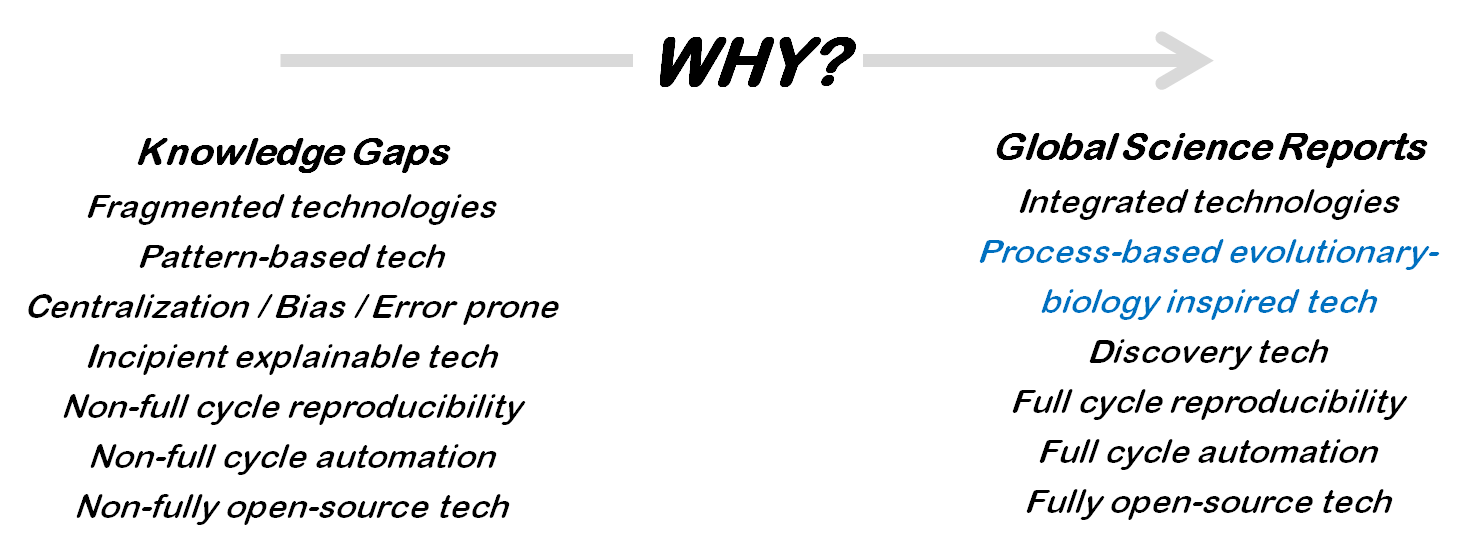
\includegraphics[width=0.75\textwidth]{Figures/Robhoot_1-1d.png}\\
  \hspace{-0.25 in}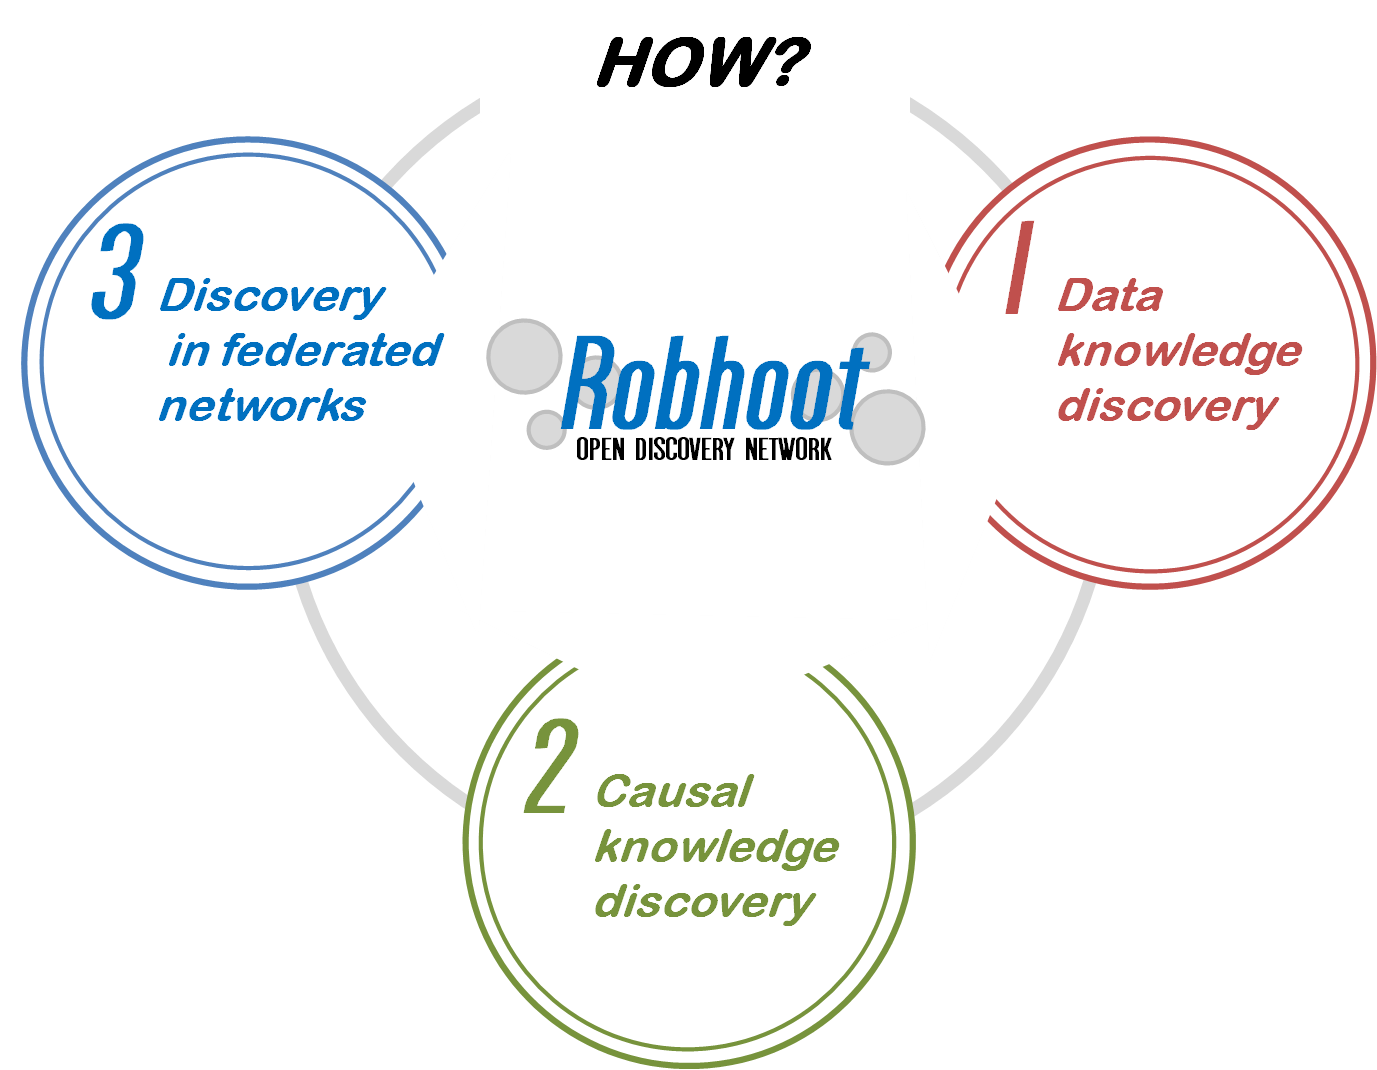
\includegraphics[width=0.75\textwidth]{Figures/Robhoot_1-2d.png}\\
  \caption*{\small {\bf Figure 1: Discovery in Evolutionary
      Biology-Inspired Federated Networks}. $\mathcal{ROBHOOT}$
    targets knowledge discovery in federated networks, networks
    composed by highly heterogeneous groups each with different
    interests in ecosystem resources, for a sustainable
    knowledge-inspired society: {\bf Top)} $\mathcal{ROBHOOT}$ targets
    global knowledge gaps for open-access reproducible global
    discovery reports. $\mathcal{ROBHOOT}$ introduces three
    science-enabled technologies: {\bf Bottom)} Evolutionary
    biology-inspired semantic and multilayer network algorithms for
    {\bf data knowledge discovery} (red), evolutionary-biology
    inspired AI-deep neural networks for {\bf causal knowledge
      discovery} (green), and evolutionary neural biology-inspired
    {\bf discovery in federated networks} (blue).}}
\end{figure}

%--------------------Summary------------------------Out of the draft -----------------------------
\begin{comment}
 The Robhoot project is trying to introduce new concepts to allow
  scientist and the public to interact in a decentralized open-access
  knowledge network to gain informed decisions when solving complex
  social, environmental and technological problems. Current
  technologies for scientific inquiry are highly fragmented and thus
  only increase robustness, reproducibility and the interactions with
  the public marginally (refs). The goal of Robhoot is to propose a
  new hybrid-technology concept combining deep learning, automation
  and distributed ledger technology with the advances of neural
  biological networks to lay the foundation for a novel open-science
  ecosystem aiming to couple predictive and knowledge power in
  contemporary societies. Robhoot is not set out to deliver a finished
  deep knowledge ledger network in the science ecosystem but provide a
  science-enabled technology in establishing a prototype
  proof-of-principle for an open public-science ecosystem.
 
\begin{table}
 %\rowcolor{pink}
\begin{tabular}{ p{6cm} | p{3cm} | p{3cm}}
  \hline \hline
  \textbf{Features} & \textbf{Science Ecosystem} &\textbf{{\bf $\mathcal{ROBHOOT}$}}\\  \hline
  Decentralization & No & Yes \\ \hline
  Full automation & No & Yes \\ \hline
  Open-access & Mostly No & Yes \\ \hline
  Immutability & No & Yes \\ \hline
  Robustness & Mostly No & Yes \\ \hline
  Reproducibility & Mostly No & Yes \\ \hline        
  Owner-Controlled assets & No & Yes \\ \hline       
  \bottomrule
\end{tabular}
\caption{{\bf $\mathcal{ROBHOOT}$} is designed to resolve desirable
  properties of science: Open-access, immutability, robustness,
  reproducibility, and owner-controlled assets. These features will be
  added during the different stages of development of the project
  (section ``Design Goals'').}
\end{table}
\end{comment}
%----------------------------------------------------------------------------------------------

\begin{comment}
\begin{table*}[ht]
 %\rowcolor{pink}
\begin{tabular}{ p{6cm} | p{11cm}}
  \hline \hline
  \textbf{Word} &\textbf{Meaning}\\  \hline
  Data knowledge discovery & Semantic discovery among data from merging heterogeneous data-sources \\ \hline
  Causal knowledge discovery & Interpretable pattern inference represented as interacting nodes and links obtained from data \\ \hline
  % Evidence-based knowledge gap & Solid scientific knowledge facing
  % constraints to be transfered to benefit society\\ \hline
  % Research-based knowledge gap & Differential access to the research
  % knowledge limiting information transfer to the society \\ \hline
  Discovery in federated networks & Novel interpretable patterns improving sustainability scenarios not present in the empirical patterns \\ \hline
  %Reproducible knowledge graph & High-resolution tracking of the research cycle to make it fully open and transparent\\ \hline
  Automation & Algorithms targeting minimal human-driven interference \\ \hline
  Knowledge inspired society & Open-access discovery to facilitate informed decisions in global sustainability challenges \\ \hline
  Neutral-knowledge generation & Reproducible reports making transparent the many sources of bias in the discovery process \\ \hline
  \bottomrule
\end{tabular}
\caption{{\bf Glossary of terms.}}
\end{table*}
\end{comment}

\subsection{Science-to-technology breakthrough that addresses this vision}

Interconnected global societies are constantly facing new challenges
that need to be rapidly addressed. In this regard, discovery
technologies providing plausible scenarios when solving complex
governance, social, environmental and technological problems are
lacking. Depite rapid advances of research platforms for data
analytics in the last decade
\citep{Melniketal:2010,Steinruecken,Modulos,Guimera2020,GoogleAI,IrisAI,easeml,datarobot,aito},
the integration of science-enabled technologies currently lack
discovery knowledge-inspired approaches impacting knowledge-inspired
societies to help responding to the rapidly changing global
sustainability challenges (Figures 1 to 3, and Tables
3.1a-c). Discovery technologies facilitating the understanding of
complex systems still present many challenges ({\bf +++}). This is
particularly relevant in global sustainability landscapes, where data
heterogeneity like varying sampling efforts, sampling methods, data
fragmentation, and lack of transparency limit our understanding of
empirical patterns to draw forecasting scenarios (Figure 2). In
addition, complex ecosystems are rooted in evolving information
processing systems driven by many factors and highly heterogeneous
living groups. Therefore, despite many years of research and insights
about complex systems (ref +++), our understanding of evolutionary
biology-inspired solutions to address complex systems is quite limited

\textcolor{red}{Discuss the relevant state-of-the-art and the extent
  of the advance the project would provide beyond this
  state-of-the-art. How will $\mathcal{ROBHOOT}$ go beyond
  state-of-the-art? $\mathcal{ROBHOOT}$ introduces evolutionary
  biology-inspired discovery in federated networks to make discovery
  an evolving feature in digital ecosytems (Figure 2). How will
  $\mathcal{ROBHOOT}$ explicitly deal with diversification and
  dimensionality when accounting for highly heterogeneous evolving
  groups and interactions? (refs about federated networks, bacterial
  consortia, federated bacteria..., artificial life, problem solving
  artificial societies, and large-scale meta-learning in the federated
  setting \citep{Dilley2016}). Describe the science-to-technology
  breakthrough, targeted by the project that would represent the first
  proof of concept of the envisioned technology.} Patterns from
knowledge-graphs are emerging at a fast pace in specific frontiers
{\bf +++}, but remains isolated from the discovery process especially
in the context of cooperative forecasting in federated networks {\bf
  +++}. $\mathcal{ROBHOOT}$ goes beyond the state-of-the-art of
knowledge-graphs by fussioning data and causal knowledge graphs, and
scalating these to evolutionary biology-inspired federated networks to
move knowledge-inspired societies towards reaching global
sustainability goals when large number heterogeneous groups share
multiple resources driven by multiple factors.

\textcolor{red}{Describe briefly the goals, how are we going to
  achieve them?} {\bf $\mathcal{ROBHOOT}$ v.1.0} deploys a data
discovery technology to generate data knowledge graphs accounting for
heterogeneous data-sources (Tables 3.1a-c and Figure
3). Data-architecture alone is not sufficent to outline predictive
scenarios in complex sustainability problems (refs +++). Therefore,
data analytics complementing data-architecture discovery is desirable
to interpret scenarios in natural and digital ecosystems. In this
regard, there are also many gaps in connecting data-architecture
assembled from many sources into rapid and automated causal knowledge
discovery. {\bf $\mathcal{ROBHOOT}$ v.2.0} introduces automated and
explainable evolutionary biology-inspired AI methods to decipher
causal knowledge discovery from open-ended modeling scenarios. Still,
rapidly drawing scenarios from a few labs limit the parameter phase
space from where the discovery process is generated. Therefore, the
scalability of fully reproducible discovery strongly depend on
cooperation and learning in large scale biology-inspired federated
networks. {\bf $\mathcal{ROBHOOT}$ v.3.0} brings knowledge discovery
to federated networks by introducing evolutionary biology
heterogeneous-neural inspired networks to obtain cooperative
forecasting scenarios from data and causal knowledge discovery
(Figures 2 and 3).

\subsection{Interdisciplinarity and non-incrementality of the research
  proposed}

\textcolor{red}{Explain why the proposed research is
  non-incremental. Describe the research disciplines necessary for
  achieving the targeted breakthrough of the project and the added
  value from the interdisciplinarity} {\bf $\mathcal{ROBHOOT}$} is a
science-enabled multi-feature technology for interpretable data-driven
discovery in federated networks (Figures 1 to 3 and Tables 1, 3.1a-c,
and 3.2a). It contains three work packages each characterized by a
mixture of research disciplines. {\bf $\mathcal{ROBHOOT}$ v.1.0} is
composed by computer scientists, evolutionary biologists, and
developers targeting novel evolutionary inspired semantic algorithms
for data discovery. This module is complemented with scientists from
complex networks taking care of quantitative methods in the data
knowledge discovery to decipher the existing gaps in data discovery
and data-architecture technologies (section 3.1.1). {\bf
  $\mathcal{ROBHOOT}$ v.2.0} is compossed by data-scientists trained
in deep learning networks and automation algorithms, theoreticians and
evolutionary biologists with expertise in modeling mechanistic and
Bayesian networks and biology-inspired neural networks,
respectively. The combination of data-scientists, theoreticians and
biologists generates a diverse team targeting synthesis between
automated and explainable evolutionary biology-inspired approaches to
decipher causal knowledge discovery from heterogeneous data-sources
(section 3.1.2). {\bf $\mathcal{ROBHOOT}$ v.3.0} combines computer
scientists and developers targeting evolutionary neural
biology-inspired models of federated networks, with social scientist,
and scientists specialized in ecology and evolutionary biology
(section 3.1.3). The complementarity of the teams in modules one to
three makes $\mathcal{ROBHOOT}$ flexible and a science-enable
functional technology in a rapidly evolving digital ecosystem
\citep{Soto-Valero2019}.

\textcolor{red}{$\mathcal{ROBHOOT}$ aims to bring global transparency
  in knowledge discovery generation by acting as an assistant or as an
  automated and reproducible discovery generator to facilitate
  sustainability goals in ecosystems. The multi-feature,
  science-enabled technology target a reduction in global knowledge
  gaps while transparently accounting for centralization
  \citep{Inhaber1977,Gunther2018}⁠⁠, bias⁠⁠ \citep{Ioannidis2005},
  error-prone \citep{Fang2011}, and non-reproducibility
  \citep{Hardwicke2018} (Figures 1 and 2 and Table 1). Improving these
  features are mostly due to the rapidly evolving digital
  ecosystem. For example, it is increasing continuously its computing
  capacity, new methods integrating automated and explainable AI are
  rapidly advancing, and their interconnection to open-source
  technologies is also rapidly occurring in the digital ecosystem {\bf
    +++}. Yet, targeting automated discovery into federated networks
  still require taking risky steps. It requires combining evolutionary
  biology-inspired solutions crossing data, causal and novel discovery
  in complex and heterogeneous data-sources and bring them to a global
  scalability...}

  \begin{comment}
  Yet, technologies with the capacity to compactly accounting for neutral,
  borderless, immutable, and open-access information in hybrid,
  trusted-untrusted peer-to-peer interactions, accounting for the
  multilayer nature of science and engineering are currently not in
  place. We have already advanced in the integration of the different
  modules, from the automated identification, retrieval and data
  integration to inference and process-based discovery. We have
  implemented a prototype for the ongoing covid-19 pandemic (section
  3.3). Each module includes state-of-the-art developments in computer
  science, complex systems, and theoretical evolutionary ecology. The
  proof- of-concept is not fully automated yet and still requires
  human intervention in module integration and the development of a
  testnet stage. Nonetheless, we are currently exploring innovative
  solutions especially in the modules of automated data discovery,
  causal-knowledge graphs, reporting, and visualization.  Producing
  such a technology will require integrating expertise from disparate
  disciplines like multilayer networks, deep learning, automation
  algorithmics, and distributed technologies. The integration of these
  disciplines will require to go beyond domain boundaries.
\end{comment}

%Renku, Fabric and gitchain.

\subsection{High risk, plausibility and flexibility of the research approach}


\begin{itemize}
\item \textcolor{red}{Explain how the research approach relates to the
    project objectives and how it is suitable to deal with the
    considerable science-and-technology uncertainties and appropriate
    for choosing alternative directions and options. (The risks and
    mitigation plan should be spelled out under the Implementation
    section).}
\end{itemize}

Knowledge-inspired societies and governance demand full research cycle
transparency, reproducibility and interpretability to inform complex
social, environmental and technological problems in the face of global
sustainability challenges. Such needs bring many technical and
functional challenges to our research proposal because obtaining
robust knowledge from integrating many parts each containing its own
set of methods can generate divergent, fragile and contradictory
outcomes. To solve this issue, {\bf $\mathcal{ROBHOOT}$} will have a
modular and flexible structure following three main work packages
(Tables 3.1a-b) with a total of ten deliverables (Table 3.1c), and
three main milestones (Table 3.2a)...


\begin{comment}
  We will develop a flexible research method focusing more in the
  algorithmic robustness of the deep ledger knowledge network than in
  the development of robust automated knowledge generation. Our
  motivation will be to provide a first proof of concept of how the
  technology works: we will sample the KGs using different deep
  learning algorithms to estimate the uncertainty of the ruled-based
  inference obtained by fitting predictions to simulated data (Goal
  G1). Accounting for the uncertainties of each of the research stages
  when sampling the KGs comes from the many distinct paths within and
  across the layers in the research cycle (Figure 1). We will test a
  variety of consensus algorithms to explore the degree of security,
  decentralization and scalability of the ledger knowledge network
  using the generated population of KGs (Goal G2). Despite our focus
  will be bias towards the side of the algorithmic robustness of the
  deep ledger knowledge network, we will develop a domain-specific
  case study, our Robhoot Open Network, to test the robustness of the
  rule-based inference obtained by fitting each of the generated KG to
  the empirical patterns (Goal G3). The high risk associated to
  robustly automate the full research cycle for producing immutable
  open knowledge is buffered to a great extend because the existing
  ecosystem of tested and reliable open-source tools: We will combine
  our own algorithms (i.e., data integration and deep learning
  algorithms for sampling and automating the KGs) with open-source
  tools like Renku, Fabric and gitchain. This open-ecosystem will
  allow us to have a flexible launching of a testnet to collect data
  to explore the security-scalability-decentralization patterns and
  the robustness of the generated KGs in the deep ledger knowledge
  network (Goal G4.)
\end{comment}



%============IMPACT====================================================
\section{Impact}

\subsection{Expected impact} 

\begin{itemize}
\item {\bf Scientific and technological contribution (to the foundation of a new future technology)}:\\
  $\mathcal{ROBHOOT}$ targets novel approaches towards sustainable
  ecosystems. One of the tasks in WP3 focus on the discovery of novel
  evolutionary-inspired algorithms to provide results for
  sustainability fisheries. Solutions around WP3 ultimately depend on
  merging WP3 with the rest of WP's in the proposal. For example, it
  is known that sustainable ecosystems strongly depend on many data
  sources collected by different groups using different technologies
  (refs +++). $\mathcal{ROBHOOT}$ discover data interactions combining
  fisheries, stakeholders, and technology data, the data knowledge
  discovery graph, as a first step towards the discovery
  process. $\mathcal{ROBHOOT}$ also infer the technological and
  environmental changes and the processes underlying the empirical
  patterns, the causal knowledge discovery graph, to provide the
  existing sustainability status in a human-disturbed
  ecosystem. Altogether, this project will lay the foundation for
  future sustainability studies. Discovery of novel
  evolutionary-inspired algorithms for biodiversity maintenance have
  been hardly been investigated in this context so far. Therefore,
  several predictors related to biodiversity, technological and social
  times series analysis will be tested and further developed to enable
  robust prediction of sustainability. The discovery of new solutions
  not observed in the empirical data, but containing the plausible
  scenarios of maintaining high values of biodiversity and
  sustainability, will be the basis for estimation of the severity of
  overfishing and sampling bias when many groups enter in commercial
  conflict of interest... Such a targeted sustainability proxies would
  be of great interest not only for the biodiversity maintenance but
  also from an economic and social point of view, as it would save
  costs for future generations. Sustainability challenges are related
  to the development of future sustainable societies, which according
  to (Organization) {\bf Keep elaborating}
  
\item {\bf Potential for future social or economic impact or market creation}:\\
  Collapse of ecosystems can lead to serious long term economic and
  ecological disfunctionalities (refs +++). However, there are not
  well established metrics for the characterization of sustainability
  in complex ecosystems. Our approach accounts for heterogeneous
  sources of data, the (evolving) mechanisms underlying technological,
  environmental and social changes required to make ecosystems
  sustainable and novel rules that could impact positively the
  maintenance of biodiversity by developing cooperative forecasting
  strategies among the many (international) groups involved. Such a
  risk assessment would not only be of great interest to the groups
  exploiting the resources, but also from an economic and ecological
  point of view, as having less bias in the field data provides more
  accurate measures from the observed time series for planning fish
  stocks for a large number of speciesq. Finally, $\mathcal{ROBHOOT}$
  contributes towards knowledge-inspired societies in need of
  radically tackling new societal and global environmental challenges:
  it provides reproducible and transparent methods for making
  sustainability goals achievable and reproducible across many sectors
  and economies.

  In the medium-term this technology may also have interesting
  applications in public and private industry. For example, access to
  discovery with cooperative forecasting might suggest new paths and
  solutions that are key to generate rapid and robust scenarios when
  facing complex problems including global sustainability challenges
  (i.e., global health, ecosystems degradation, biodiversity loss,
  etc). First, evolutionary biology-inspired AI algorithms deciphering
  open-ended search of interpretable mechanisms underlying the
  targeted complex systems for private and public industry facing
  highly heterogeneous data sources. Second, cooperative forecasting
  challenges existing fragmented responses to emergent global
  sustainability problems by compactly offering reproducible
  forecasting emerging from many-to-many human and machine cooperative
  discovery, and third, open-access explainable and automated
  information generation account for global data-arquitecture allowing
  individuals and companies to address scenarios of future strategies
  in highly fluctuating local and global market conditions.

\item {\bf Impact on transparency and reproducibility}:\\
  Decision making and governance at local, regional and global scales
  require access to transparent and reproducible information
  containing the interpretable factors and their plausibility to
  explain the empirical patterns. In this regard, the
  $\mathcal{ROBHOOT}$ consortium brings together excellent partners
  from the fields of computer science, neurobiology, complex system,
  biology, social sciences, evolutionary ecology and including one SME
  focusing on reproducibility, automation, visualization and reporting
  along its whole developmental life cycle (Dissemination plan below
  and Figure 3).


  At the same time, all groups composing the consortium
  exhibit a long-standing experience interdisciplinary research across
  the boundaries of the individual disciplines (Figure 3). The
  subsection on related projects shows that this is a novel
  constellation in Europe and possibly worldwide (section 4). This
  consortium is also at the leading edge of developing novel
  evolutionary biology-AI inspired solutions to automation and
  reproducibility in complex systems facing sustainability challenges.
  
\item {\bf Ecosystem health impact}:\\
  Ecosystem sustainability and ecosystem health are usually used as
  metaphors to describe the mechanisms that maintain functional and
  diverse systems and the condition of an ecosystem,
  respectively. Ecosystem sustainability and condition can vary as a
  result of many disturbances like fire, flooding, drought,
  extinctions, invasive species, climate change, mining,
  overexploitation in fishing, farming or logging, chemical spills,
  and a host of other reasons. $\mathcal{ROBHOOT}$ focus on novel
  discovery solutions for ecosystems under a varying degree of
  disturbances. $\mathcal{ROBHOOT}$ introduces a case study for
  overexploited ocean ecosystems when highly heterogeneous social
  groups with different interests exploit limited and shared
  resources. Thus, $\mathcal{ROBHOOT}$ is a technology designed to
  provide novel discovery solutions paths for ecosystem
  sustainability, improving the underlying discovery paths that allow
  draw novel connections between ecosystem sustainability and
  ecosystem health. This feature aligns to the EU Reflection paper
  towards a Sustainable Europe by 2030 focusing on the need of
  investing in sustainable growth and spur action by goverments,
  institutions and citizens, leading the way for the rest of the world
  using the UN's Sustainable Development Goals (SDGs). Specifically,
  $\mathcal{ROBHOOT}$ can be seen as an horizontal enabler for the
  sustainability transition to make Europe sustainable by 2030. It
  introduces evolutionary biology- and artificial
  intelligence-inspired solutions to benefit ecosystem health and
  people’s lives and work. By being able to process large amounts of
  heterogeneous data instantaneously, artificial intelligence and
  evolutionary-biology inspired solutions have the potential to
  significantly increase productivity in environmental sustainability
  and ultimately make informed decisions to enhance food security
  \citep{EUcommission}.
  
\item {\bf Building leading research and innovation capacity across Europe}:\\
  This consortium brings together excellent partners from the fields
  of computer science, machine learning, deep learning networks,
  neurobiology, complex systems, experimental biology, biology and
  evolutionary ecology and in particular evolutionary biology-inspired
  federated networks both from a theoretical and an experimental point
  of view, Physics, theory and applications of complex systems in
  social networks and one highly innovative science-based
  reproducibility, automation, reporting and communication focusing on
  sustainability solutions. Many of the components of the consortium
  are first-time participants to FET under Horizon 2020 (Section
  4). The use of advanced evolutionary biology-inspired and complex
  networks-based analyses to characterize and predict novel discovery
  in systems formed by heterogeneous and evolving groups and
  interactions combined with the implementation of intelligent
  learning discovery in federated networks and the development of a
  reproducible and automated protocol user friendly interface go much
  beyond the current state-of-the-art in science-based discovery
  technologies. All consortium partners exhibit a long-standing
  experience in interdisciplinary research across the boundaries of
  the individual disciplines (Figure 3). The subsection on related
  projects shows that this consortium is at the leading edge of
  innovation and interdisciplinarity (Tables 3.1a-c). A significant
  value proposition of the project is to increase the research on
  large-scale sustainable federated networks where many heterogeneous
  agents share resources embedded in complex ecosystems. This will
  produce valuable information and data about how federated networks
  work under broad set of socio-ecological scenarios, similar to
  natural ecosystems consoritiums where many paths produce coexistence
  of heterogneous poulations and high biodiversity (refs ++). It is
  important to consider that all ecosystems facing many human
  pressures are all across the world and discovery technologies
  facilitating the solutions in large-scale federated networks could
  inspire new developments improving our understanding of
  sustainability at global scale. For in-home, we also expect an
  explosion of discovery knowledge approaches and future publications,
  which will place Europe at the top of sustainability in federated
  networks.

  Moreover, in WP3, we propose the generation of a web-based
  sustainability discovery portal that will allow researchers, NGO,
  managers and the public to train students in the discovery process
  to manage over-exploited ecosystems, allowing to scale up the number
  of people participating in the sustainability process by an order of
  magnitude thus mobilising forward thinking researchers and excellent
  young researchers to work together and explore what may become a new
  technology paradigm in sustainability research. Members of the
  consortium already have experience in generating such types of
  training tools that are currently available online (check github
  repository RobhooX). This approach would provide an unprecedented
  capability for the access to a multitude of people interested in
  sustainability discovery tools that will result in facilitating
  consensus and a valuable source of information for science-enabled
  technologies in ecosystem sustainability and management.
\end{itemize}
 
  
\subsection{Measures to maximize impact} 
\label{sec:maximize-impact}

\subsubsection{Dissemination and exploitation of results}

%\label{sec:dissemination-exploitation}
%\instructions{
\begin{itemize}
\item {\bf The Plan for diseminating and exploiting the project
    results} $\mathcal{ROBHOOT}$ allocates three research groups along
  its whole developmental life cycle to guarantee dissemination,
  transparency and easy exploitation of the technology {\bf
    (when)}. {\bf (what)} The three milestones of the project, data
  knowledge discovery, causal knowledge discovery and discovery in
  federated networks (Table 3.2a) will be fully automated and
  reproducible to facilitate visualization, reporting and full
  scalability. {\bf (who)} Automated discovery will be implemented
  along Bayesian machine scientist to facilitate open-ended search
  during the development of the three milestones (Deliverable D3.4,
  $\mathcal{BSM}$, $\mathcal{ICREA}$, Tables 3.1a-b). Reproducible
  knowledge discovery graphs will be developed in the Renku
  open-source software (Deliverable D3.5, $\mathcal{DATAR}$ by the
  Swiss Data Science Center, $\mathcal{SDSC}$). Visualization and
  reporting will be fully implemented in the Julia computing language
  for its speed and unique features (Deliverable D3.6,
  $\mathcal{VISUR}$, by $\mathcal{DESANTANA}$. Codes will be available
  in the public git \href{https://github.com/RobhooX/Robhoot}{Robhoot}
  repository. Having the whole developmental life cycle as
  reproducible and automated knowledge discovery graphs facilitates
  the reuse and the dissemination of the technology as a whole in any
  platform and OS. Full reproducibility, automation, visualization and
  reporting provide to $\mathcal{ROBHOOT}$ legal and financial
  transparency and reproducibility in social governance a feature for
  easy replication of the discovery process by third parties, a
  property that can be used to facilitate reporting for governance
  public policy, NGO, society and thinktank in the face of local and
  global sustainability challenges. {\bf why, how and which journals,
    conferences and with which preliminary results}.
  
\item All the data, codes and outputs generated during
  $\mathcal{ROBHOOT}$ development will be open access stored in public
  git repositories. The project will collect data from many sources
  (i.e., fisheries, environmental and social data, technology data).
  generate data knowledge discovery graphs, causal knowledge graphs
  and the data and algorithms generated from the discovery in
  federated networks for the exploration of the Seas case study
  (Deliverable D1.2, $\mathcal{DATAX}$, D2.3, $\mathcal{DIX}$, and
  D3.3, $\mathcal{DIFEX}$, respectively). {\bf Keep elaborating}
  \end{itemize}
  %\emph{You will need an appropriate consortium agreement to manage
  % (amongst other things) the ownership and access to key knowledge
  % (IPR, data etc.). Where relevant, these will allow you,
  % collectively and individually, to pursue market opportunities
  % arising from the project's results.} \\
  % \emph{The appropriate structure of the consortium to support
  % exploitation is addressed in section 3.3.}\\
  % \emph{Self-archiving (also called 'green' open access) means
  % that the published article or the final peer-reviewed manuscript
  % is archived by the researcher - or a representative - in an
  % online repository before, after or alongside its
  % publication. Access to this article is often - but not
  % necessarily - delayed (``embargo period''), as some scientific
  % publishers may wish to recoup their investment by selling
  % subscriptions and charging pay-per-download/view fees during an
  % exclusivity period.

  \subsubsection{Communication activities}

  \begin{itemize}
  \item The full open-source developmental life cycle strategy of
    reproducibility, automation, and reporting generation of
    $\mathcal{ROBHOOT}$ targets the search of societal relevance and
    long-term economic impact of open and transparent
    science. Underlying to this strategy is to build support for
    future research and innovation funding, by ensuring uptake of
    results within the scientific community, and opening up potential
    business opportunities for novel products or services, and
    potentially contributing to better decision-making processes and
    valuable input for public policies
    formulation. $\mathcal{ROBHOOT}$ has very general dissemination
    targets, from scientists and decision-makers, to the business
    community and the public. $\mathcal{ROBHOOT}$'s general
    dissemination measures will focus on project results and
    stakeholder engagement (stakeholder consultation processes;
    workshops to raise awareness, etc.) through:\\
    \hspace{0.15 in}. The project website is to be set up within the
    first three months of the project. There is already a public git
    \href{https://github.com/RobhooX/Robhoot}{Robhoot} repository.\\
    \hspace{0.15 in}. Up to date information material, e.g. brochures,
    presentationslides, will be distributed at events to increase awareness about the $\mathcal{ROBHOOT}$ project.\\
    \hspace{0.15 in}. General other publication means will be used
    such as newspapers, YouTube, TV and radio, social networks as well
    as
    targeted mailing lists (e.g., evodir, AI-worldwide).\\
    \hspace{0.15 in} Scientific publications for the scientific
    community. We will target high-level journals with open access (i.e., Science, Nature Communication, etc.)\\
    \hspace{0.15 in}. The consortium will visit conferences in the
    related scientific fields and interdisciplinary conferences in
    order to interactively present and discuss our results with others
    researchers, groups and institutions. Among other activities, the
    consortium will organize special sessions at several conferences
    in different countries. Additionally, some targeted, specific
    dissemination actions will be considered: We will organize
    hackatons and robhacks activities to attract multipliers and
    developers from the open-source community to the community who
    engage in data processing and build hybrid evolutionary
    biology-inspired and AI algorithms. This will be achieved by a
    “traveling salesman” approach using personal visits and
    invitations to demonstrate how $\mathcal{ROBHOOT}$ works. At the
    end of the project we will organize a workshop specifically on
    ``Evolutionary-biology AI inspired solutions for global
    sustainability challenges'' for disseminating our results to a
    broad set of groups and experts in fields related to global
    sustainability for assessing future exploitation
    potential, inviting partners from academia as well as industry.\\
    \hspace{0.15 in}. $\mathcal{ROBHOOT}$ will launch a testnet to
    help disseminate the main results of discovery in federated
    networks (Section 3.1.3). The launch will have invited NGO’s and
    GO across disciplines and social, economical and technological
    sectors. The $\mathcal{ROBHOOT}$ Open Discovery Network will be
    launched as a Biodiversity and sustainability open discovery
    network to offer the solutions for the exploration of the Seas
    case study and to integrate additional public databases and data
    collections into the open discovery network to facilitate NGOs,
    GOs and other organizations transparency, reproducibility, and
    governance in Biodiversity management.

\item $\mathcal{ROBHOOT}$ strictly adheres to the Open Access Policy
  of the Commission and all publishable (non-protected) results will
  follow the green or gold OA policy. Software as well as hardware
  protocols will be made openly available through standard computer
  science repositories. The $\mathcal{ROBHOOT}$ public git repository
  is already active
  \href{https://github.com/RobhooX/Robhoot}{Robhoot}. Data (measured
  data), as such, will not be acquired by
  $\mathcal{ROBHOOT}$. Open-source codes and analysis of standardized
  inputs/outputs and software will be made public through an online
  platform with the aim of converting it in The Reference Point for
  any future research in knowledge discovery. Open access to
  publications will be granted under the terms and conditions laid
  down in the Grant Agreement, in accordance with the Rules for
  participation and dissemination in Horizon 2020. The beneficiaries
  will deposit an electronic copy of the published version or the
  final manuscript accepted for publication of a scientific
  publication relating to foreground in an institutional or
  subject-based repository at the moment of publication, e.g., via the
  OpenAIRE portal (www.OpenAIRE.eu). In addition, beneficiaries will
  make their best efforts to ensure that this electronic copy becomes
  freely and electronically available to anyone through this
  repository (i.e., that it becomes “open access”): immediately, if
  the scientific publication is published “open access”, i.e., if an
  electronic version is also available free of charge via the
  publisher, or within 6 months of publication.
  \end{itemize}

\section{Implementation}

A technology deciphering data and causal knowledge discovery to tackle
global sustainability challenges is highly informative by itself, but
a diverse group of scientists across Europe have decided to connect
discovery and sustainability broadly. We want to advance cooperative
discovery in the global digital ecosystem. To this end, the
$\mathcal{ROBHOOT}$ consortium aims at integrating data and causal
knowledge discovery, into evolutionary-biology and neural-inspired
federated networks to provide cooperative forecasting scenarios for
sustainability challenges. $\mathcal{ROBHOOT}$'s goals are developed
along three main work packages, three milestones and twelve
deliverables (Tables 3.1a-c).

\begin{figure}[h!]
  %\centering
   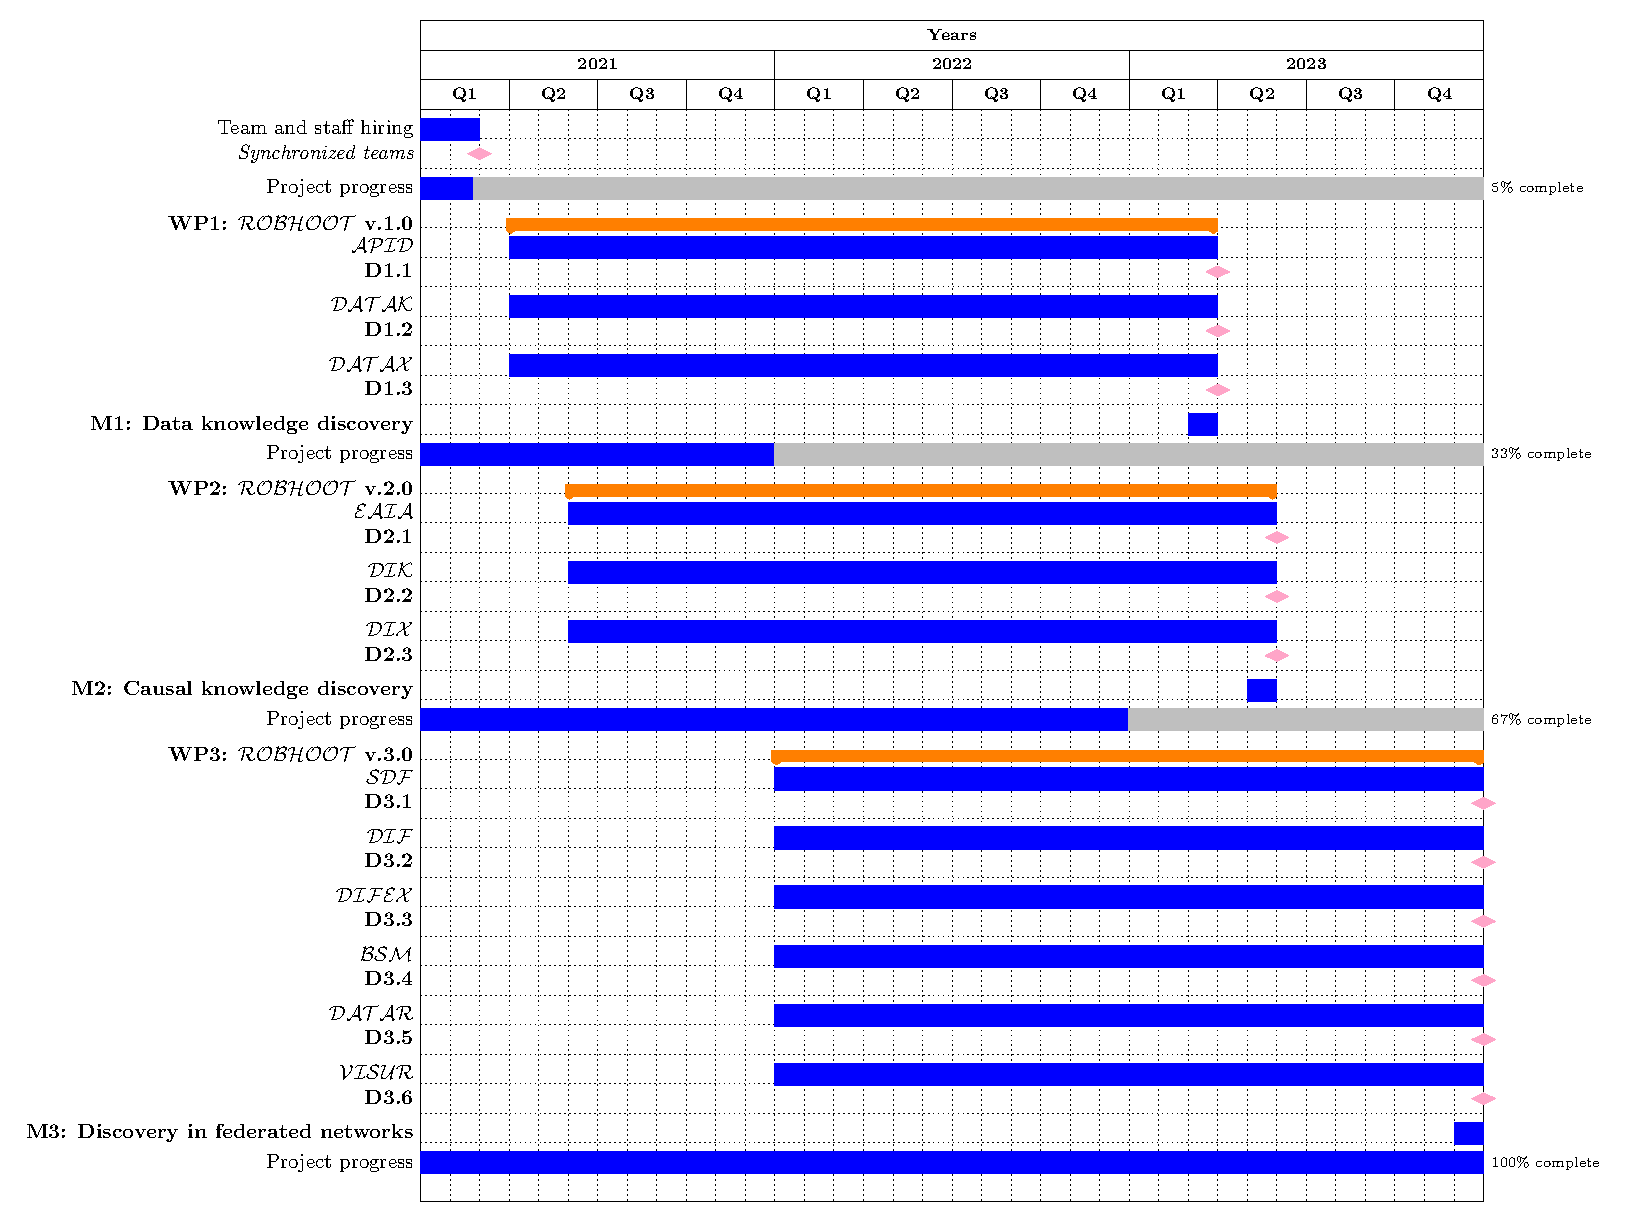
\includegraphics[width=1\textwidth]{Figures/GanttChart.pdf}
   \caption*{{\small {\bf Table 3.1a: $\mathcal{ROBHOOT}$ Gantt
         Chart}: Work package one, {\bf $\mathcal{ROBHOOT}$ v.1.0}
       introduces deliverables {\bf D1.1} to {\bf D1.3} for data
       knowledge discovery for the exploration of the Seas case study
       (Figure 2). {\bf $\mathcal{ROBHOOT}$ v.2.0} introduces
       deliverables {\bf D2.1} to {\bf D2.3} for causal knowledge
       discovery for the exploration of the Seas, and {\bf
         $\mathcal{ROBHOOT}$ v.3.0} introduces {\bf D3.1} to {\bf
         D3.6} for discovery in federated networks for the exploration
       of the Seas. Reproducibility, automation, visualization and
       reporting deliverables are developed along the full life cycle
       of $\mathcal{ROBHOOT}$.}}
\end{figure}

  
\subsection{Research methodology and work plan , work packages,
  deliverables}

\subsubsection{{\bf WP1: $\mathcal{ROBHOOT}$ v.1.0}: \\ Data Knowledge
  Discovery}

\textcolor{blue}{Fortuna and Egu\'iluz:: Storing and organizing much
  of the rapidly accumulating scientific information in rigorous,
  principled ways, so that finding what we want and understanding what
  is already known has became exhausting, frustating, stressful and
  increasingly costly experiences (refs +++). For information to be
  usable, it should be stored and organized in ways that allow us to
  access it, to analyze it, to annotate it and to relate it to other
  information and make the whole process reproducible. The first step
  is, therefore, to translate the scientific knowledge stored in
  existing databases to machine-readable format. Only a few databases
  are semantically anotated (e.g. , gene ontology database). This is
  because ontology development is time-consuming, requires expert
  knowledge and community commitment, and is ideally paired with
  data-driven research that iteratively checks the soundness of the
  ontology as it simultaneously seeks discovery. Software tools for
  mapping and linking the terms between different ontologies are still
  to be developed, although Semantic Web technologies are included in
  programs such as the U.S. National Science Foundation's proposed
  CyberInfrastructure (refs +++).\\
  The approach that we are adopting, therefore, begins with the raw
  data, ontologically interprets and transforms the data in order to
  extract its semantics and express such semantics in
  ontologies. These ontologies are then mapped to a graph-based data
  architecture. Neo4j is the implementation technology that we have
  currently chosen to adopt. The main reasons for adopting a graph
  database to persist the ontological models are: (1) the flexibility
  that a graph structure provides in implementing any modelling
  paradigm and (2) the scalability it provides in terms of organizing
  and accessing massive amounts of data.\\
  Next, we need to integrate the diverse and heterogeneous large-scale
  data sets that we have semantically annotated previously since they
  originate from distinct communities of scientists in separate
  subfields. This will be achieved in large part through the adoption
  of novel technologies. The few technologies and available tools are
  still quite limited for many scientists and only a few research
  groups have tried to apply it on real data (refs +++). It is rather
  difficult to ask simple questions like, for example, which human
  diabetes-related proteins are located in the nucleus of the cell and
  are interacting with proteins related to pancreatic cancer (refs ++
  example on sustainability?). Such question requires the integration
  of data from multiple sources. New approaches are needed to make
  progress in this direction.\\
  (edited from here) API discovery technologies to build robust and
  scalable automated data-driven discovery is an existing need
  \citep{Fan2012,Staar2018}. Technologies around building database are
  particularly relevant to move beyond explainable (or interpretable)
  Artificial Intelligence technologies and for discovery in global
  emergency or sustainability landscapes where new questions and
  scenarios are constantly emerging and new data is constantly being
  added to a large pool of servers \citep{Futia2020}. Building
  database from a large pool of heterogeneous data, however, comprises
  a series of privacy requirements, formats, dimensions, biases and
  spatiotemporal resolution that constraint data integration and
  discovery \citep{Openstreetmap,Bluecloud,HOT,Elixir}. Fortunately,
  standard protocols to automate API discovery, semantic knowledge
  extraction, and ETFs algorithms are rapidly advancing
  \citep{Fan2012,APISGURU,OpenKnowledgeFoundation}, and overall
  different types of semantic technologies are rapidly emerging in the
  context of integrating many datasets into data knowledge graphs
  \citep{KGcovid19}. Yet, technologies focusing on novel evolutionary
  semantic knowledge extraction algorithms to build data knowledge
  graphs from many heterogeneous data-sources that can be rapidly
  integrated into interpretable technologies are not currently in
  place \citep{Futia2020}} (\textcolor{red}{Fortuna: make clear how
  evolutionary biology-inspired semantic knowledge extraction
  algorithms might work}. $\mathcal{RH}$v.1.0 explores evolutionary
biology-inspired semantic algorithms around heterogeneous API
data-discovery along three main deliverables (Deliverables D1.1,
$\mathcal{APID}$, to D1.3, $\mathcal{DATAX}$, Figure 3 and Tables
3.1a-c). $\mathcal{RH}$v.1.0 delivers a data knowledge discovery graph
from heterogeneous data-sources for the exploration of the Seas case
study (Figure 2). $\mathcal{RH}$v.1.0 explores evolutionary
biology-inspired rules using sematic algorithms to discover API and
interactions that can be added to the exploration of the Seas
database. The exploration of the Seas database started in 1965 and it
actually has around 9 million entries, 1612 species, 20 countries and
11 sampling methods (Figure 2). $\mathcal{RH}$v.1.0 will expand it
with Fishery data using the
(\href{https://globalfishingwatch.org/}{global fishing watch}),
species interactions and social and stakeholders groups with different
interests within each of the countries involved in the international
exploration of the Seas.}


 %Word package description
\begin{table}[h!]
\begin{center}
  {\footnotesize \begin{tabular}{|m{3cm} || m{12cm} || m{1cm}|}
    \hline\hline\hline
    \rowcolor{lightpink!30}
    {\bf Work package} & {\bf Lead Beneficiary} & \\
    \hline
    \rowcolor{piggypink!20}
    {\bf WP Title} & {\bf $\mathcal{ROBHOOT}$ v.1.0} &  \\
    \hline
    \rowcolor{piggypink!20}
    {\bf Participant number} & {\bf 1, 2} & \\
    \hline
    \rowcolor{piggypink!20}
    {\bf Short name of participant} & {\bf $\mathcal{EBD-CSIC}$ (1), $\mathcal{IFISC-CSIC}$ (2)} & \\
    \hline
    \rowcolor{piggypink!20}
    {\bf Person Month per participant} & 1 and 2:(12 months $\times$ 0.25 (25\% allocated time) == 3 (Provisional) & \\
    \hline
    \rowcolor{piggypink!20}
    {\bf Start month} & {\bf 4} & \\
    \hline
    \rowcolor{piggypink!20}
    {\bf End month} & {\bf 28} & \\
    \hline
    \rowcolor{piggypink!20}
    {\bf Objectives} & Evolutionary biology-inspired semantic and multilayer networks algorithms for data knowledge discovery & \\
    \hline
    \rowcolor{piggypink!20}
    {\bf Description} & Patterns from diverse data-sources for novel knowledge discovery & \\
    \hline
    \rowcolor{piggypink!20}
    {\bf Deliverables} & {\bf D1.1 ($\mathcal{APID}$}, Delivery month: 27, Lead: 1): Interaction data discovery from evolutionary biology-inspired semantic algorithms
                         {\bf D1.2 ($\mathcal{DATAK}$}, Delivery month: 27, Lead: 2): Data knowledge discovery mixing evolutionary semantic and multilayer network algorithms
                          {\bf D1.3 ($\mathcal{DATAX}$}, delivery month: 28, Lead: 1 and 2): Data knowledge discovery for the exploration of the Seas federated network & \\
    \hline\hline\hline
    \rowcolor{piggypink!20}
    {\bf WP Title} & {\bf $\mathcal{ROBHOOT}$ v.2.0} &  \\
    \hline
    \rowcolor{piggypink!20}
    {\bf Participant number} & {\bf 3, 4, and 5} & \\
    \hline
    \rowcolor{piggypink!20}
    {\bf Short name of participant} & {\bf $\mathcal{FISHEC-EAWAG}$ (3), $\mathcal{SIAM-EAWAG}$ (4), $\mathcal{TARTU}$ (5)} & \\
    \hline
    \rowcolor{piggypink!20}
    {\bf Person Month per participant} & 3, 4, and 5:(12 months $\times$ 0.25 (25\% allocated time) == 3 (Provisional) & \\
    \hline
    \rowcolor{piggypink!20}
    {\bf Start month} & {\bf 6} & \\
    \hline
    \rowcolor{piggypink!20}
    {\bf End month} & {\bf 30} & \\
    \hline
    \rowcolor{piggypink!20}
    {\bf Objectives} & Evolutionary biology-inspired AI-neural networks algorithms for causal knowledge discovery & \\
    \hline
    \rowcolor{piggypink!20}
    {\bf Description} & Interpretable knowledge extraction for causal knowledge discovery & \\
    \hline
    \rowcolor{piggypink!20}
    {\bf Deliverables} & {\bf D2.1 ($\mathcal{EAIA}$}, Delivery month: 29, Lead: 3 and 4): Evolutionary biology-inspired AI algorithms        
                         {\bf D2.2 ($\mathcal{DIK}$}, Delivery month: 29, Lead: 4 and 5): Evolutionary biology-inspired algorithms for interpretable knowledge discovery              
                         {\bf D2.3 ($\mathcal{DIX}$}, Delivery month: 30, Lead: 3, 4 and 5): Causal knowledge discovery for the exploration of the Seas case study & \\
    \hline \hline\hline
    \rowcolor{piggypink!20}
    {\bf Title} & {\bf $\mathcal{ROBHOOT}$ v.3.0} &  \\
    \hline
    \rowcolor{piggypink!20}
    {\bf Participant number} & {\bf 6, 7, 8, 9 and 10} & \\
    \hline
    \rowcolor{piggypink!20}
    {\bf Participants} & {\bf $\mathcal{IT-EAWAG}$ (6), $\mathcal{UNIGRAZ}$ (7), $\mathcal{ICREA}$ (8), $\mathcal{SDSC}$ (9), $\mathcal{DESANTANA}$ (10) & \\
    \hline
    \rowcolor{piggypink!20}
    {\bf Person Month per participant} &  6, 7, 8, 9 and 10:(12 months $\times$ 0.25 (25\% allocated time) == 3 (Provisional)  & \\
    \hline
    \rowcolor{piggypink!20}
    {\bf Start month} & {\bf 12} & \\
    \hline
    \rowcolor{piggypink!20}
    {\bf End month} & {\bf 36} & \\
    \hline
    \rowcolor{piggypink!20}
    {\bf Objectives} & Evolutionary neural-inspired knowledge discovery in federated networks & \\
    \hline
    \rowcolor{piggypink!20}
    {\bf Description} & Automated discovery knowledge graphs in federated networks & \\
    \hline
    \rowcolor{piggypink!20}
    {\bf Deliverables} & {\bf D3.1 ($\mathcal{SDF}$}, Delivery month: 34, Lead: 6): Sharing knowledge discovery in federated networks
                         {\bf D3.2 ($\mathcal{DIF}$}, Delivery month: 34, Lead: 7): Neural biology-inspired discovery in federated networks 
                         {\bf D3.3 ($\mathcal{DIFX}$}, Delivery month: 34, Lead: 6 ad 7): Neural biology-inspired discovery for the exploration of the Seas federated network
                         {\bf D3.4 ($\mathcal{BSM}$}, Delivery month; 36, Lead: 8): Automated Bayesian scientist for knowledge discovery in federated networks
                         {\bf D3.5 ($\mathcal{DATAR}$}, Delivery month: 36, Lead: 9): Reproducible knowledge discovery in federated networks
                         {\bf D3.6 ($\mathcal{VISUR}$}, Delivery month: 36, Lead: 10): Visualizing and reporting of knowledge discovery in federated networks & \\
    \hline\hline\hline
                 \end{tabular}
                 }
\end{center}
\caption*{{{\bf Table 3.1b  $\mathcal{ROBHOOT}$ work package description}: Work package,
    Title, Participants, Person Months per participant, Start and End
    month, Objectives, Description and deliverables of each Work
    Package.}}
\end{table}

\subsubsection{{\bf WP2: $\mathcal{ROBHOOT}$ v.2.0}: \\
  Causal Knowledge Discovery}

Particularly relevant in Earth, Ecosystem and Sustainability science,
the rapid progress of AI as an automated and explainable technology
(\citep{OHare2015,Gil2019,Cranmer2019,Guimera2020,Real2020,Futia2020},+++)
will increase our ability to make stronger inferences about future
sustainability challenges and solutions
\citep{Reichstein}. $\mathcal{RH}$v.2.0 explores evolutionary
biology-AI-inspired solutions to infer the causal interactions
underlying heterogeneous and complex multidimensional datasets
(Deliverables D2.1, $\mathcal{EAIA}$ to D2.3, $\mathcal{DIX}$, Tables
3.1a-c).


\textcolor{blue}{Baity, Vicente, Mel\'ian:
  $\mathcal{RH}$v.2.0 introduces evolutionary biology-AI-inspired
  algorithms for the exploration of the Seas case study to ask
  questions around the drivers and their connections to the
  sustainability of the Oceans (Figure 2). For this, we need to
  identify the actors, e.g., species, threats like fishing activity,
  environental and habitat data, and then infer causal connections
  among all of them. As an illustration, the use of different Gears
  across countries affects the spatial and temporal samplings and the
  distribution of fish species. The consequence of the distribution of
  abundance/catches of Megrim and Haddock is strongly affected by the
  choice of gears by the Irish and the Spanish fleet (Figure 2). A
  group represents a set of actors with multiple traits. In this
  context, groups can be represented with evolving environmental and
  technological traits. This can be formally described as a
  distribution-fishery cooperation-competition matrix,
  $\mathcal{C}^{2}$, as follows:
  \vspace{0.1 in}\\
\begin{center}
  $\mathcal{C}^2$ = \bordermatrix{~ &
    $\mathcal{F}^{i}_{\mathcal{A}_{g},\mathcal{B}_{g}}(c)$ &
    $\mathcal{F}^{i}_{\mathcal{A}_{g},\mathcal{B}_{g}}(nc)$ \cr
    $\mathcal{D}^{i}_{\mathcal{A}_{g},\mathcal{B}_{g}}(c)$ &
    $c(\varphi)$ & $c(\Phi), nc(\gamma_{A_{g}},\gamma_{B_{g}})$ \cr
    $\mathcal{D}^{i}_{\mathcal{A}_{g},\mathcal{B}_{g}}(nc)$ &
    $nc(\Phi_{A_{g}},\Phi_{B_{g}}), c(\gamma)$ &
    $nc(\phi_{A_{g}},\phi_{B_{g}})$ \cr}, \vspace{0.2 in}
\end{center}
\\
where $\mathcal{D}$, $\mathcal{F}$, $i$, $\mathcal{A}_{g}$,
$\mathcal{B}_{g}$, c and nc, represent distribution map and fishery of
species $i$, group $g$ within country $\mathcal{A}$ and $\mathcal{B}$,
cooperation and non-cooperation, respectively. We will explore
evolutionary biology-inspired functions representing environmental and
technological traits with different degrees of complexity in the
$\mathcal{C}^2$ matrix: If the two groups within the countries
cooperate, $c(\varphi)$, then the environmental and technological rate
change, $\varphi$, is syncrhonized between groups to evolve towards
decreasing Gear bias and make distribution maps and the fishery
sustainable. On the other side, if the two groups decide not to
cooperate, $nc(\phi_{A_{g}},\phi_{B_{g}})$, then there is
environmental and technological rate change, $\phi_{A_{g}}$ and
$\phi_{B_{g}}$ with each group following changes of their own gears,
the GOV for the Ireland group and the Baka Gear for Spain group,
independently of the other and as a function of their fishery
interest. There is no interest in decreasing bias in species
distribution maps making fishery non sustainable in this case. In the
last two scenarios groups enter in cooperation for the distribution
map of species $i$, but not in the fishery
($c(\Phi), nc(\gamma_{A_{g}},\gamma_{B_{g}})$), or they do cooperate
in the Fishery for species $i$ but not for the distribution map of
species $i$ ($nc(\Phi_{A_{g}},\Phi_{B_{g}}), c(\gamma)$). The
situation for cooperation in the distribution maps follows agreements
between the two groups to technological changes in the Gear but still
preserving their GOV and the Baka Gears for
fisheries. $\mathcal{RH}$v.2.0 search causal knowledge discovery for
the exploration of the Seas containing 9 million entries, 1612 species
(around 50 variables and traits per species), around 20 countries and
11 sampling methods (Figure 2). The search contrasts scenarios from
evolutionary biology-AI-inspired algorithms combining them to
automated Bayesian machines ensuring the search, the evaluation of
models, trading-off complexity, fitting to the data and quantify
resource usage (Deliverable D3.4,
$\mathcal{BSM}$)\citep{Guimera2020,Steinruecken}. Causal knowledge
graphs connect automated and explainable AI throughout prediction and
knowledge power (Figure 2).} \textcolor{red}{Baity, Vicente, Mel\'ian:
Make more clear how the evolutionary-biology-AI inspired modeling will
be implemented: The explanation above is a first glimpse to be
improved}

\begin{comment}
  I have trouble understanding the details of the KG in fig. 2: are
  there only edges between neightboring columns of nodes (if not,
  perhaps you want to draw this differently, arranging the clusters of
  nodes around the perimeter of a circle, like in the plot of
  connections between brain areas (see att.).

  Can you also give an example what knowledge a concrete edge in this
  KG could encode?  You write that is supposed to represent a causal
  KG. How does this affect the content of the edges?

  It would be very helpful if you could also give for this fish domain
  some concrete examples for the KGs that are considered in WP1, 2, 3,
  and the new methods and insights that these WPs are intended to
  produce for this fish example? This would help me to get an idea of
  the methods that would be needed for this.
\end{comment}


   \vspace{0.15 in}
   \begin{figure}[h!]%{r}{0.35\textwidth}
     \begin{center}
       \vspace{-0.25 in}
     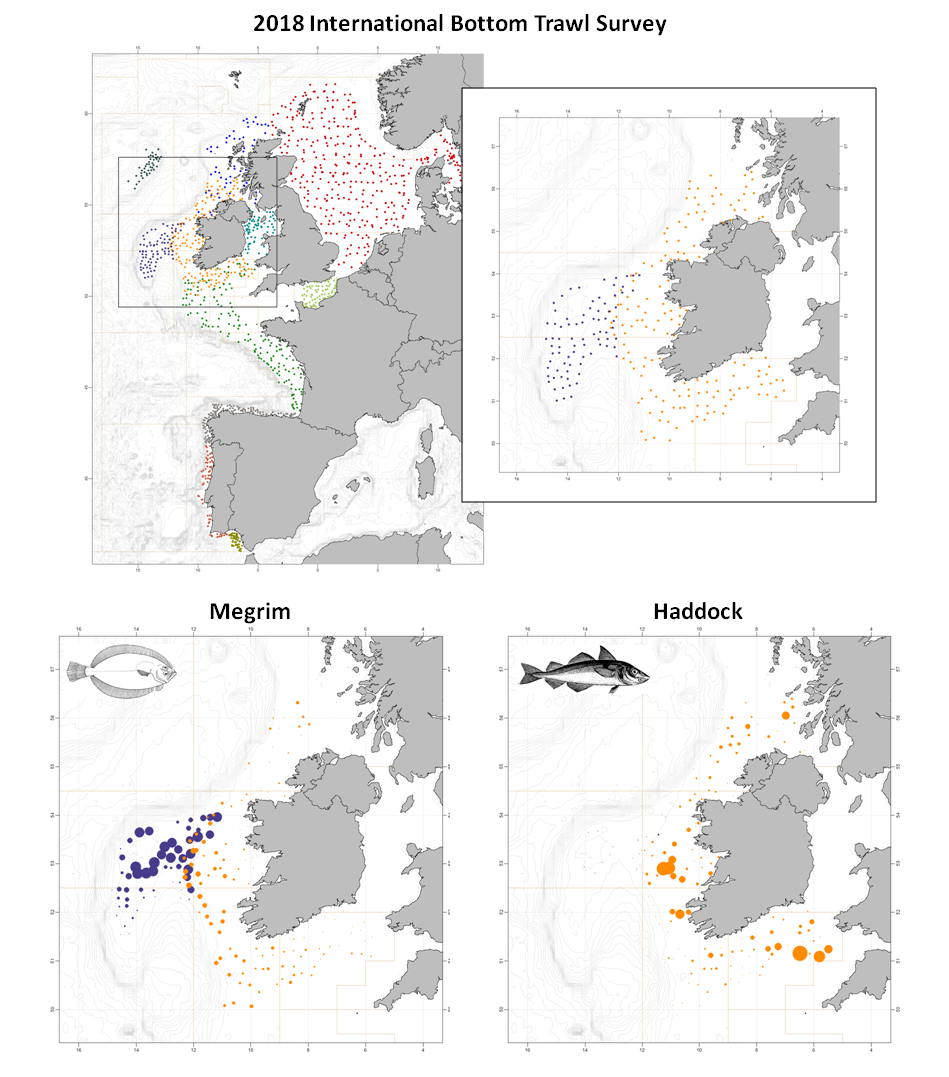
\includegraphics[width=0.6\textwidth]{Figures/Figura.png}
     \\
     \vspace{-0.15 in}
     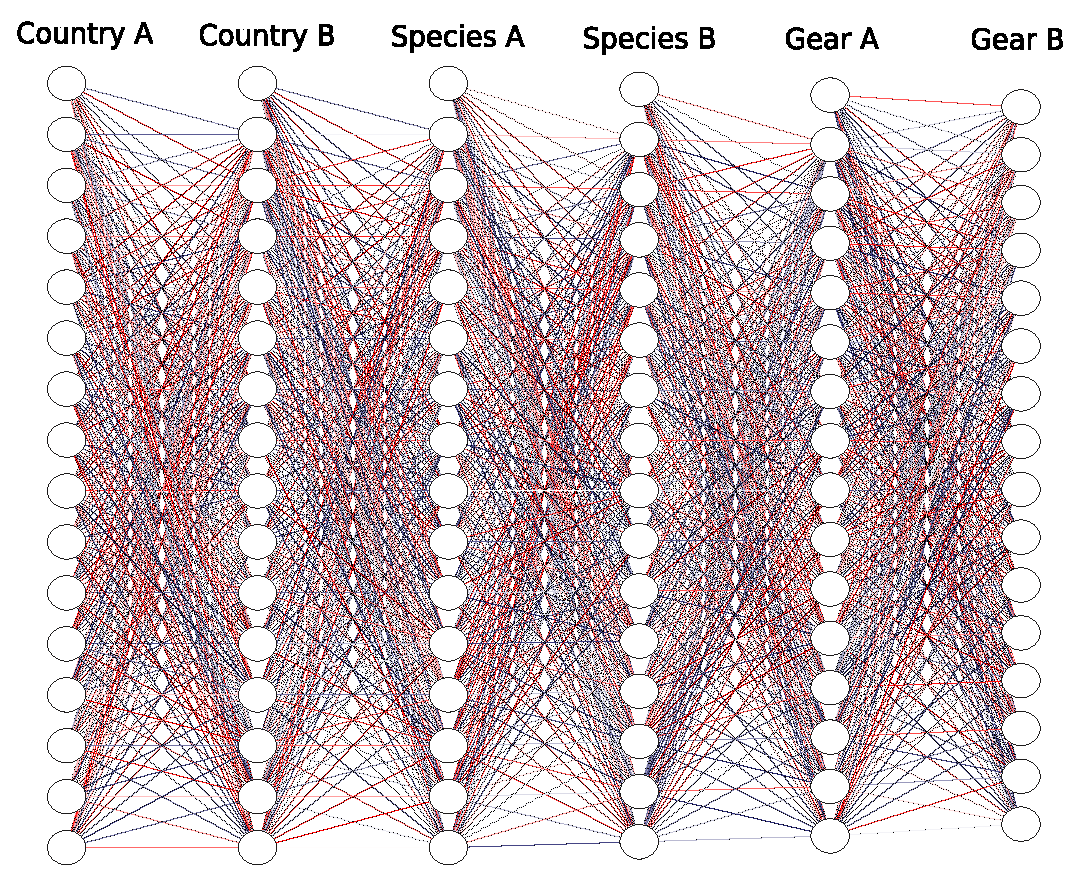
\includegraphics[width=8cm,height=6cm]{Figures/CKG.pdf}
     \vspace{-0.15 in}
     \caption*{\small {\bf Figure 2: Causal Knowledge Discovery for
         Sustainable Ecosystems}. {\bf Top}) The Irish Ground Fish
       Survey (IE-IGFS, Orange) and the Spanish Survey on the
       Porcupine Bank (SP-PORC, Blue) were part of the 2018
       International Bottom Trawl Survey, coordinated by the
       International Council for the Exploration of the Sea
       \citep{ices}. Ireland and Spain use different Gears: The GOV
       gear has a larger vertical opening (Ireland, 3-4 m) respect to
       the Baka used on the Porcupine Bank (Spain, 2-3 m). This makes
       catchability different for fish species, such as Megrim
       ($Lepidorhombus$ $whiffiagonis$, {\bf Center left}) and Haddock
       ($Melanogrammus$ $aeglefinus$, {\bf Center right}), in which
       both countries have very different commercial
       interests. Haddock is a species of the cod family, highly
       prized in northern Europe, while Megrim is a species of
       flatfish, consumed largely in Spain and France. Spain catches
       Megrim better than Haddock and viceversa for Ireland. This
       generates a strong bias in the distribution maps (compare
       Megrim vs. Haddock map, Center) with potential implications for
       biodiversity management and sustainability in natural
       ecosystems. {\bf Bottom} Causal knowledge discovery graph
       representing the 2-countries, 2-species and 2 gears for the
       example above. The whole data set for 2018 contains 11
       countries, 461 fish especies (approx. 200k individuals
       sampled), and 5 gears. Each country, species and gear is
       composed by many nodes: For example country contains fishery,
       environmental agency, stakeholders, etc. Species contains
       size-classes, habitat preference, species interactions,
       etc. Red and blue links mean competition and cooperation links
       connecting each pair of nodes.}
\end{center}
  \end{figure}

%Deliverable table  
\begin{table}[h!]
\begin{center}
  \begin{tabular}{|m{1.9cm} || m{1.25cm} || m{1.75cm} || m{0.75cm} || m{4.85cm} || m{1.2cm} || m{1cm} || m{1cm}|}
  \hline\hline
  \rowcolor{lightpink!30}
  {\bf $\mathcal{ROBHOOT}$ v.X.X} & {\bf Deliver. number} & {\bf Deliver. name} & {\bf WP} & {\bf Name Lead} & {\bf Type} & {\bf Disem.} & {\bf Date} \\
  \hline\hline
  \rowcolor{piggypink!20}
  {\bf v.1.0} & {\bf D1.1} & $\mathcal{APID}$ & WP1 & {\bf $\mathcal{EBD-CSIC}$} & OT & PU & 27 \\
  \hline\hline
  \rowcolor{piggypink!20}
  {\bf v.1.0} & {\bf D1.2} & $\mathcal{DATAK}$ & WP1 & {\bf $\mathcal{IFISC-CSIC}$} & OT & PU  & 27 \\
  \hline\hline
  \rowcolor{piggypink!20}
  {\bf v.1.0} & {\bf D1.3} & $\mathcal{DATAX}$ & WP1 & {\bf $\mathcal{EBD-IFISC-CSIC}$} & R,DEC & PU  & 28 \\
    \hline\hline
 \rowcolor{piggypink!40}
  {\bf v.2.0} & {\bf D2.1} & $\mathcal{EAIA}$ & WP2 & {\bf $\mathcal{FISHEC-EAWAG}$} & OT & PU & 29 \\
  \hline\hline
  \rowcolor{piggypink!40}
  {\bf v.2.0} & {\bf D2.2} & $\mathcal{DIK}$ & WP2 & {\bf $\mathcal{SIAM-EAWAG}$, $\mathcal{TARTU}$} & OT & PU  & 29 \\
  \hline\hline
  \rowcolor{piggypink!40}
    {\bf v.2.0} & {\bf D2.3} & $\mathcal{DIX}$ & WP2 & {\small {\bf $\mathcal{FISHEC-SIAM-EAWAG}$, $\mathcal{TARTU}$}} & R,DEC & PU & 30 \\
    \hline\hline
   \rowcolor{piggypink!60}
  {\bf v.3.0} & {\bf D3.1} & $\mathcal{SFN}$ & WP3 & {\bf $\mathcal{IT-EAWAG}$} & OT & PU & 34 \\
  \hline\hline
   \rowcolor{piggypink!60}
  {\bf v.3.0} & {\bf D3.2} & $\mathcal{DIF}$ & WP3 & {\bf $\mathcal{UNIGRAZ}$} & OT & PU & 34 \\
  \hline\hline
  \rowcolor{piggypink!60}
    {\bf v.3.0} & {\bf D3.3} & $\mathcal{DIFEX}$ & WP3 & {\bf $\mathcal{IT-EAWAG}$, $\mathcal{UNIGRAZ}$} & R,DEC & PU & 34 \\
  \hline\hline
   \rowcolor{piggypink!80}
  {\bf v.3.0} & {\bf D3.4} & $\mathcal{BSM}$ & WP3 & {\bf $\mathcal{ICREA}$} & OT & PU  & 36 \\
    \hline\hline
     \rowcolor{piggypink!80}
  {\bf v.3.0} & {\bf D3.5} & $\mathcal{DATAR}$ & WP3 & {\bf $\mathcal{SDSC}$} & OT & PU  & 36 \\
    \hline\hline
     \rowcolor{piggypink!80}
  {\bf v.3.0} & {\bf D3.6} & $\mathcal{VISUR}$ & WP3 & {\bf $\mathcal{DESANTANA}$} & OT & PU  & 36 \\
\hline\hline
  \end{tabular}
\end{center}
\caption*{{{\bf Table 3.1c List of Deliverables}: {\bf
      $\mathcal{ROBHOOT}$} contains three main work packages and
    twelve deliverables: {\bf $\mathcal{ROBHOOT}$ v.1.0} span from
    Month 4 to 28. Deliverable {\bf D1.3 ($\mathcal{DATAX}$)}
    generates the data knowledge discovery for the exploration of the
    Seas case study. Work package {\bf $\mathcal{ROBHOOT}$ v.2.0} span
    from Month 6 to 30. Deliverable {\bf D2.3 ($\mathcal{DIX}$)}
    generates the causal knowledge discovery for the exploration of
    the Seas case study, and {\bf $\mathcal{ROBHOOT}$ v.3.0} span from
    Month 12 to 36, bringing the deliverable {\bf D3.3
      ($\mathcal{DIFEX}$)}, discovery in neural biology-inspired
    federated networks for the exploration of the Seas case
    study. Deliverables {\bf D3.4} to {\bf D3.6}, Bayesian space
    models, {\bf $\mathcal{BSM}$}, reproducible knowledge discovery,
    {\bf $\mathcal{DATAR}$}, and visualization and reporting, {\bf
      $\mathcal{DESANTANA}$}, respectively, fully guarantee
    automation, reproducibility and visual reporting for the whole
    life cycle of $\mathcal{ROBHOOT}$. OT: Other (software/technical
    diagram, etc), R: Document report, DEC: website, press and media
    activity, videos and PU: Public fully open.}}
\end{table}

\subsubsection{{\bf WP3: $\mathcal{ROBHOOT}$ v.3.0}: \\
  Discovery in Federated Networks}

Integrating data and causal knowledge graphs provide a mechanistic
understanding of how much cooperation vs. competition is occurring in
our exploration of the Seas case study. However, causal knowledge
graphs are not enough if they only represent isolated contributions
and can not ``learn to learn'' to find novel, emergent solutions in
neural biology-inspired networks composed by highly heterogeneous groups. In
this regard, federated objects can be seen as ``neural networks''
containing many types of heterogeneous nodes with varying degrees of
learning in the context of heterogeneity, connectivity and firing
probabilities \citep{Maass2014,Maass2015}. Technologies in digital
ecosystems around federated networks are scarce and mostly focus on
decentralization, scalability and security fronts
\citep{Golem2016,Dilley2016,Durov2017,Androulaki2018,OceanProtocolFoundation2018,BigchainDBGmbH2018}. In
the science ecosystem, only a few applications of open decentralized
technologies exist \citep{Gunther2018}. Yet, the discovery of novel
algorithms in biology-inspired federated networks for cooperative
forecasting of global sustainability problems when heterogeneous
groups learn and share from each other is currently not in place.

Recent studies have shown the importance of evolutionary search of
mathematical and symbolic operations as building blocks to discover ML
algorithms (\citep{Real2020,Guimera2020}). Evolutionary
biology-inspired search for algorithmic discovery can help to decipher
how interactions among heterogeneous groups evolve and learn to solve
complex sustainability problems. For example, evolutionary dynamics
can explore open-ended language of models with varying trait evolution
functions to discover biologically inspired solutions in
multidimensional systems (\citep{Real2020},+++). $\mathcal{RH}$v.3.0
deploys sharing discovery knowledge graphs, D3.1, $\mathcal{SFN}$,
into biology-inspired federated networks accounting for heterogeneous
agents to discover novel biology-inspired solutions for the
exploration of the Seas federated network (Deliverables D.3.1,
$\mathcal{SFD}$ to D.3.3, $\mathcal{FIDEX}$, Tables
3.1a-c). Evolutionary algorithms might trigger novel algorithmic
findings, the discovery knowledge graphs, and \textcolor{blue}{von
  Haldow, Maass:: $\mathcal{RH}$v.3.0 introduces ``Cooperative
  Forecasting'' as evolutionary biology-inspired neural learning
  algorithms for the discovery of new solutions in large federated
  networks (Tables 3.1a-c). $\mathcal{RH}$v.3.0 search for how
  learning among interacting heterogeneous groups discover
  evolutionary algorithms and in our exploration of the Seas case
  study this can be represented as follows: Now the focus is on
  cooperative learning to discover new solutions. For example, how
  learning from the most distant strategies in the technological and
  environmental traits can make distribution catchability maps
  similar. Groups can now be represented not only as environmental and
  technological traits, but with evolving learning traits as a
  function of the distance between each pair of groups sharing
  resources. This can be formally
  described as a distribution-fishery cooperation learning matrix $\mathcal{C}^2$, as follows: \vspace{0.2 in}\\
\begin{center}
  $\mathcal{C}^2$ = \bordermatrix{~ & $\mathcal{F}^{i}_{\mathcal{A}_{g},\mathcal{B}_{g}}(c)$ & $\mathcal{F}^{i}_{\mathcal{A}_{g},\mathcal{B}_{g}}(nc)$ \cr
    $\mathcal{D}^{i}_{\mathcal{A}_{g},\mathcal{B}_{g}}(c)$ & $c(\varphi,\mathcal{L}_{d})$ & $c(\Phi,\mathcal{L}_{d}), nc(\gamma_{A_{g}},\gamma_{B_{g}})$ \cr
    $\mathcal{D}^{i}_{\mathcal{A}_{g},\mathcal{B}_{g}}(nc)$ & $nc(\Phi_{A_{g}},\Phi_{B_{g}}), c(\gamma,\mathcal{L}_{d})$ & $nc(\phi_{A_{g}},\phi_{B_{g}})$ \cr}, \vspace{0.2 in}
\end{center}
\\
where $\mathcal{D}$, $\mathcal{F}$, $i$, $\mathcal{A}_{g}$,
$\mathcal{B}_{g}$, c and nc, represent distribution map and fishery of
species $i$, group $g$ within country $\mathcal{A}$ and $\mathcal{B}$,
cooperation, and non-cooperation, respectively, as in
$\mathcal{ROBHOOT}$ v.2.0. In addition, we introduce learning
functions depending of the distance between two groups,
$\mathcal{L}_{d}$. We will search evolving learning functions that can
be coupled to environmental and technological traits with different
degrees of complexity in the $\mathcal{C}^2$ matrix: If the two groups
within the countries are sufficiently distant, then learning functions
play a role to cooperate, $c(\varphi, \mathcal{L}_{d})$, and the
environmental and technological rate change, $\varphi$, strongly
depend on learning between the interacting groups making distribution
maps and the fishery more sustainable.\\
(Write from here how the learning scenario can enter in the
non-cooperative strategies) On the other side, if the two groups
decide not to cooperate, $nc(\phi_{A_{g}},\phi_{B_{g}})$, then there
is environmental and technological rate change, $\phi_{A_{g}}$ and
$\phi_{B_{g}}$ with each group following changes of their own gears,
the GOV for the Ireland group and the Baka Gear for Spain group,
independently of the other and as a function of their Fishery
interest. There is no interest in decreasing bias in species
distribution maps making fishery non sustainable in this case. In the
last two scenarios groups enter in cooperation for the distribution
map of species $i$, but not in the Fishery
($c(\Phi), nc(\gamma_{A_{g}},\gamma_{B_{g}})$), or they do cooperate
in the Fishery for species $i$ but not for the distribution map of
species $i$ ($nc(\Phi_{A_{g}},\Phi_{B_{g}}), c(\gamma)$). The
situation for cooperation in the distribution maps follows agreements
between the two groups to technological changes in the Gear but still
preserving their GOV and the Baka Gears for
Fisheries. $\mathcal{RH}$v.2.0 search discovery knowledge graphs for
the exploration of the Seas (Figure 2) containing 9 million entries,
1612 species, 15 countries and 11 sampling methods contrasting
predictions from evolutionary biology-inspired algorithms and
complements it with automated Bayesian machines ensuring the process
is fully automated to facilitate search, and evaluation of models
(Deliverable D3.4, $\mathcal{BSM}$) \citep{Guimera2020,Steinruecken},
and communication of the full approach in public repositories (Section
Impact).}
 
Our understanding of the outcomes from evolved information processing
systems formed by highly heterogeneous groups, a kind of large-scale
meta-learning in the federated setting \citep{Dilley2016}, is
currently quite limited. Therefore, new science-enabled approaches
accounting for information processing with diversification of
heterogeneous and highly dimensional systems in federated networks are
required to develop science-enabled technologies where heterogeneous
agents with different interests find (non optimal)
solutions. $\mathcal{RH}$v.3.0 connects discovery knowledge graphs to
biology-inspired federated netwoks to study the properties of
cooperative forecasting and strong inference in the face of global
sustainability and biodiversity challenges (Figure 2 and Tables
3.1.a-c).

\begin{comment}
\begin{table*}[ht]
 %\rowcolor{pink}
\begin{tabular}{ p{3.5cm} | p{14cm}}
  \hline \hline
  \textbf{Feature} &\textbf{$\mathcal{ROBHOOT}$}\\  \hline
  Long-term vision & Global open-access to a fully reproducible knowledge-generation inspired technology \\ \hline
  Breakthrough scientific and technological target & Collapsing evidence- and research-based knowledge gaps for a sustainable knowledge-inspired society\\ \hline
  Novelty & Science-based technology emerging from targeted algorithmic discovery at the interface of multilayer networks, knowledge graphs, deep-learning, and consensus mechanisms\\ \hline
  Foundational & Neutral-knowledge inspired technology for an emerging open science of science and science-society research disciplines \\ \hline
  High-risk & Adapted to explore new terrirories into the open-science-technology-society interface ecosystem \\ \hline
  Interdisciplinarity & Hybridizing expertise from distributed computing and deep learning to multilayer networks and the ecology and evolution of natural and digital ecosystems (Table 1) \\ \hline
  \bottomrule

\end{tabular}
\caption{{\bf $\mathcal{ROBHOOT}$} features along its developmental stages.}
\end{table*}
\end{comment} 



  \begin{comment}
    %\centering
  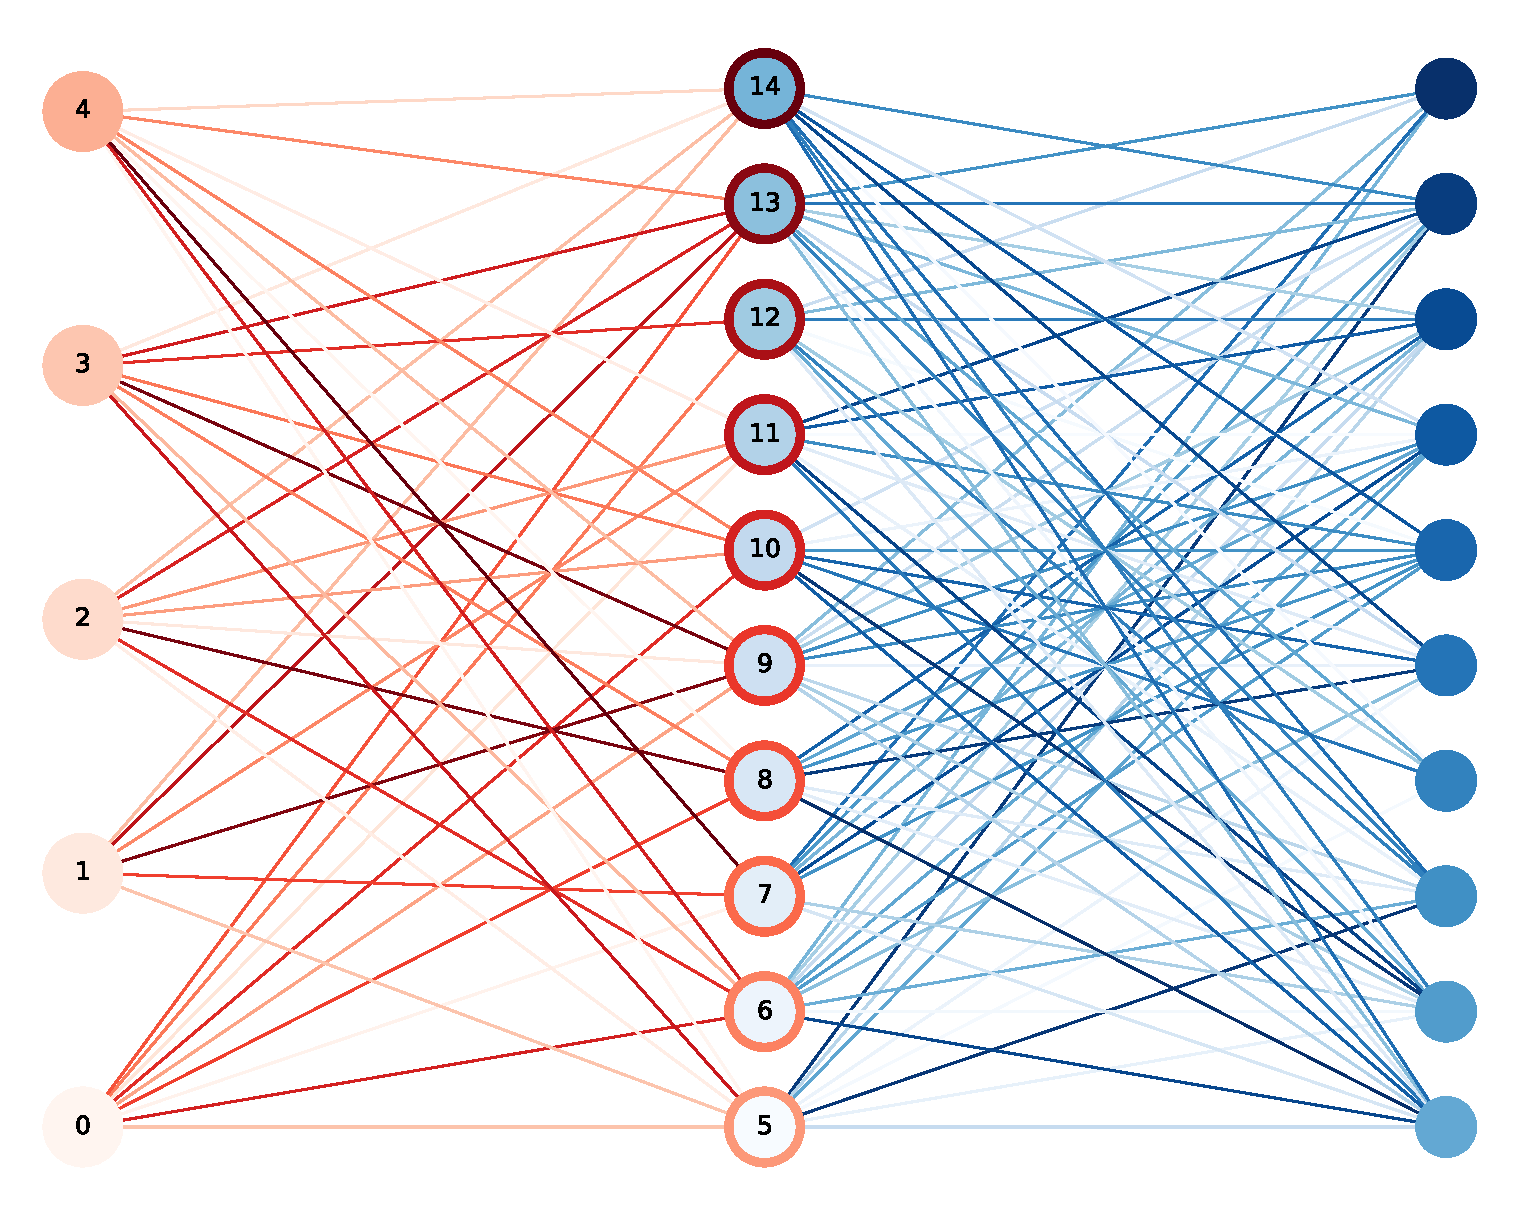
\includegraphics[width=0.45\textwidth]{Figures/FigureRobhoot.pdf}
 
  {\small {\bf Figure 3: Robhoot in Digital Ecosystems}: {\bf Left
      column}: {\bf $\mathcal{ROBHOOT}$ v.1.0} representing the
    research cycle as nodes from number 0 to 4: Data integration (0),
    Complexity Reduction (1), Inference (2), Validation (3), and
    Visualization(4)). {\bf Central column}: Nodes representing the
    research cycle in the left column are connected to open-source
    software in the digital ecosystem. Connections with node number 0
    in the left column can, for example, represent the ETLs
    open-source software interactions required to generate the {\bf
      Universal ETLs} module. The same meaning applies to the
    different nodes of the left column. {\bf Right column}: Each node
    represents a report meaning there is a reporting gradient
    generated by the connections to the open-source software from
    where each report is generated only using a subset of the research
    layers and open-source software.}
\end{comment}


\subsection{Management structure, milestones and procedures}

\begin{itemize}
  \item \textcolor{red}{Describe the organisational structure and the
      decision-making (including a list of milestones (table 3.2a))}
\item \textcolor{red}{Explain why the organisational structure and
  decision-making mechanisms are appropriate to the complexity and
  scale of the project.}
\item \textcolor{red}{Describe any critical risks, relating to project
    implementation, that the stated project's objectives may not be
    achieved. Detail any risk mitigation measures. Please provide a
    table with critical risks identified and mitigating actions (table
    3.2b) and relate these to the milestones.}
\end{itemize}


Advisory board covering the weakest parts of the proposal -- mention here

%Milestone table  
\begin{table}[h!]
\begin{center}
  \begin{tabular}{|m{1.75cm} || m{2.5cm} || m{2.5cm} || m{2.4cm} || m{6cm}|}
   \hline\hline
   \hline\hline
  \rowcolor{lightpink!30}
  {\bf Milestone number} & {\bf Milestone name} & {\bf Related work package(s)} & {\bf Due data (months)} & {\bf Verification} \\
   \hline\hline
   \rowcolor{piggypink!20}
  {\bf M1} & {\bf Data knowledge discovery} & WP1 & 28 & OS-Software,Paper/Conf.,Main-website &
  \hline\hline
  \rowcolor{piggypink!30}
  {\bf M2} & {\bf Causal knowledge discovery}  & WP2 & 30 & OS-Software,Paper/Conf.,Main-website &
  \hline\hline
   \rowcolor{piggypink!40}
  {\bf M3} & {\bf Discovery in federated networks} & WP3 & 36 & OS-Software,Paper/Conf.,Main-website &
  \hline\hline
\hline\hline
  \end{tabular}
\end{center}
\caption*{{{\bf Table 3.2a: List of Milestones}: {\bf
      $\mathcal{ROBHOOT}$ v.1.0} to {\bf v.3.0} span from month 4 to
    28, 6 to 30 and 12 to 36, respectively, to generate the ``Data
    knowledge discovery'', the ``Causal knowledge discovery'' and the
    ``Discovery in federated networks'' for the exploration of the
    seas case study. Verification for each milestone combines
    Open-Source software, papers and/or conference and a main website
    featuring reproducible, automated, visual and interpretable
    discovery.}}
\end{table}

%critical risks for implementation
\begin{table}[h!]
\begin{center}
  \begin{tabular}{|m{4.75cm} | m{2.5cm} | m{6.5cm}|}
    \hline
  \rowcolor{lightpink!30}
  {\bf Description of risk} & {\bf Work package} & {\bf Proposed risk mitigation measures} &
   \hline\hline
   \rowcolor{piggypink!20}
  \centerline {\bf Medium} & \centerline {\bf WP1} & Ontology-semantic algorithms as an alternative to evolutionary semantic algorithms to infer interactions among distinct data to build the data knowledge discovery as a general case and for the exploration of the Seas & 
  \hline\hline
  \rowcolor{piggypink!20}
  \centerline {\bf Medium} & \centerline {\bf WP1}  & Alternative to full automation for data ontologies, which are the algorithms? &
  \hline\hline
   \rowcolor{piggypink!20}
  \centerline {\bf Low} & \centerline {\bf WP1} & Implementation of static multilayer metrics to characterize data knowledge discovery graphs &
  \hline\hline
   \rowcolor{piggypink!40}
  \centerline {\bf Medium} & \centerline {\bf WP2} & Alternatives to evolutionary-biology-AI-inspired algorithms: modular approach& 
  \hline\hline
  \rowcolor{piggypink!40}
  \centerline {\bf Low} & \centerline {\bf WP2}  & Alternative to full automation for causal discovery, constraints to evolving functions &
  \hline\hline
   \rowcolor{piggypink!40}
  \centerline {\bf Low} & \centerline {\bf WP2} & Alternatives to causal discovery automation for the exploration of the Seas &
 \hline\hline
   \rowcolor{piggypink!60}
  \centerline {\bf Low} & \centerline {\bf WP3} & Alternatives to evolutionary neural biology-inspired algorithms in federated networks & 
  \hline\hline
  \rowcolor{piggypink!60}
  \centerline {\bf Low} & \centerline {\bf WP3}  & Automation of cooperative discovery and forecasting  &
  \hline\hline
   \rowcolor{piggypink!60}
  \centerline {\bf Medium} & \centerline {\bf WP1-WP3} & Modular alternatives to ``full reproducibility'' connecting the three work packages &
 \hline\hline
  \rowcolor{piggypink!60}
  \centerline {\bf Medium} & \centerline {\bf WP1-WP3} & Modular alternatives to ``full automation'' connecting the three work packages &
\hline\hline  
  \end{tabular}
\end{center}
\caption*{{{\bf Table 3.2b: Critical risks for implementation}:
    $\mathcal{ROBHOOT}$ contains risks along its three main WPs and
    milestones. $\mathcal{RH}$v.1.0 with milestone ``Data knowledge
    discovery'' has three main risks related to evolutionary semantic
    algorithms, data discovery automation, and the multilayer metrics
    to characterize data knowledge graphs. $\mathcal{RH}$v.2.0 with
    milestone ``Causal knowledge discovery'' has three main risks
    related to evolutionary-biology-AI inspired algorithms, causal
    discovery automation, and discovery automation for the exploration
    of the Seas case study. $\mathcal{RH}$v.3.0 with milestone
    ``Knowledge discovery in federated networks'' has X main risks
    related to evolutionary neural biology-inspired algorithms, its
    automation, its interactions to x and y for full reproducibility
    and visualization and reporting.}}
\end{table}



  \subsection{Consortium as a whole}
  {\bf $\mathcal{ROBHOOT}$} is a science-enabled multi-feature
  technology designed with a highly modular structure. Modularity
  allows to gain module functionality while maintaining
  cross-functional features among the different parts to produce a
  science-enabled interdisciplinary technology (Figure 3, WP one to
  three and milestones one to three, red, green and blue,
  respectively): {\bf Data knowledge discovery}'s team requires skills
  in evolutionary biology, evolutionary computation, computer science
  and the physics of complex systems (Section 3.1.1, Table 3.2a and
  Figure 3). {\bf $\mathcal{ROBHOOT}$ v.1.0} work package mixes
  complementary expertise in semantic algorithms, evolutionary
  computation algorithms and multilayer network metrics to create
  novel evolutionary-biology inspired ontology anotations when merging
  heterogeneous data-sources into one data knowledge discovery. {\bf
    $\mathcal{EBD-CSIC}$}\footnote{Miguel Fortuna} team takes care of
  data knowledge graphs introducing novel evolutionary semantic
  algorithms to discover ontologies and interactions among many
  data-sources (Deliverable D1.1, {\bf $\mathcal{APID}$}, Tables
  3.1a-c). {\bf $\mathcal{IFISC-CSIC}$}\footnote{Victor Egu\'iluz}
  team focuses on multilayer network modularity, community detection
  and decentralization metrics for pattern detection in data knowledge
  discovery (Deliverable D1.2, {\bf $\mathcal{DATAK}$}, Tables
  3.1a-c). {\bf $\mathcal{EBD-CSIC}$} and {\bf $\mathcal{EBD-IFISC}$}
  teams will join efforts to merge evolutionary semantic algorithms
  and multilayer network metrics to produce the data knowledge
  discovery for the exploration of the Seas case study (Deliverable
  D1.3, {\bf $\mathcal{DATAX}$}, Tables 3.1a-c and Figure 3 Milestone
  one in red).

  {\bf $\mathcal{ROBHOOT}$ v.2.0}'s team composed by {\bf
    $\mathcal{EAWAG-SIAM}$}\footnote{Marco Baity}, {\bf
    $\mathcal{TARTU}$}\footnote{Raul Vicente, to be confirmed} and
  {\bf $\mathcal{EAWAG-FISHEC}$\footnote{Carlos Meli\'an}} fussion
  Evolutionary biology, AI Algorithms and deep learning networks, the
  ``Evolutionary biology-inspired AI algorithms'' approach
  (Deliverable D2.1, {\bf $\mathcal{EAIA}$}, Table 3.1a-c and Figure
  3, green). The overall goal of this milestone is to connect
  evolutionary biology mechanisms to deep learning networks to
  generate a {\bf Causal knowledge discovery} technology to make
  patterns interpretable (Deliverable D2.2, {\bf $\mathcal{DIK}$}),
  Section 3.1.2, Table 3.2.a-c and Figures 2 and 3). The team for this
  milestone add inter-module complementarity expertise to {\bf
    $\mathcal{ROBHOOT}$ v.1.0}'s team: Now the skills focus on
  data-scientists trained in deep learning networks and evolutionary
  biologists with expertise in evolutionary ecology theory and
  evolutionary-inspired networks (section 3.1.2 and Figure 3,
  green). Milestone two generates a causal knowledge discovery for the
  exploration of the Seas initially containing 9 million entries, 1612
  species using around 11 sampling methods and more than 15 countries
  (Deliverable D2.3, {\bf $\mathcal{DIX}$}, Figures 2 and 3,
  green). Interdisciplinarity in $\mathcal{ROBHOOT}$ enters not only
  at the intra-module development stage, but also at the inter-module
  stage where causal knowledge discovery and evolutionary
  biology-inspired AI algorithms might form the basis for the
  emergence of interdisciplinarity breakthrough ideas reflected in the
  highly complementarity skills of the consortium. The first two
  modules in {\bf $\mathcal{ROBHOOT}$} contain researchers from
  Estonia, Spain, Switzerland.

  The {\bf $\mathcal{ROBHOOT}$} consortium wants to advance the
  rapidly evolving digital ecosystem by making cooperative discovery a
  fundamental feature of it. For this purpose, a science-enabled data
  and causal knowledge discovery technology is not enough if they stay
  isolated from a discovery technology embedded in larger and scalable
  networks. To discover novel scenarios for ecosystem sustainability,
  {\bf Discovery in federated networks} should learn to learn from
  heterogeneous data-sources in the context of evolutionary neural
  biology-inspired algorithms. To achieve scalability for the
  discovery in federated networks, neural-inspired protocols in
  federated networks is the excellency feature of {\bf
    $\mathcal{ROBHOOT}$ v.3.0} (section 3.1.3). {\bf
    $\mathcal{ROBHOOT}$ v.3.0}'s team composed by {\bf
    $\mathcal{EAWAG-IT}$}\footnote{Harald von Waldow} and {\bf
    $\mathcal{UNIGRAZ}$}\footnote{Wolfgang Maass}, develop protocols
  for sharing data and causal knowledge discovery and neural
  biology-inspired federated networks, respectively. The team forming
  {\bf $\mathcal{ROBHOOT}$ v.3.0} also requires contrasting skills:
  First, developers working in sharing and security protocols to
  guarantee scalable transfer of data and causal knowledge
  discovery. Second, social scientists, computer scientists, and
  neurobiologists in collaboration to developers aiming to explore the
  role of evolving neural biology-inspired solutions accounting for
  heterogeneous data-sources in federated networks. {\bf
    $\mathcal{ROBHOOT}$ v.3.0} is a fundamental stepping-stone for
  developing ``Cooperative Forecasting'': it first guarantees data and
  causal knowledge discovery are shareable objects. Then these objects
  represent the basis for discovery of novel paths that increase
  sustainability goals produced in the different nodes of a network
  that interact and learn from each other to find better forecasting
  scenarios at a global scale. {\bf $\mathcal{ROBHOOT}$ v.3.0}'s
  implements heterogeneous groups of (cooperating and competing)
  neurons in federated networks for making cooperative forecasting a
  standard global property of $\mathcal{ROBHOOT}$ (Deliverable D3.2,
  {\bf $\mathcal{DIF}$}, Tables 3.1a-c). Milestone three generates
  discovery in federated networks for the exploration of the Seas to
  provide populations of scenarios satisfying biodiversity and
  sustainability maintenance while guaranteeing commercial interest of
  many interacting groups and stakeholders within and among countries
  (Deliverable D3.3, {\bf $\mathcal{DIFEX}$}, Figure 3,
  blue). $\mathcal{ROBHOOT}$ v.3.0} contain researchers from
Switzerland and Austria. $\mathcal{ROBHOOT}$ architecture aims to
guarantee strong communication and impact along its whole life cycle
and development. The team formed by the {\bf $\mathcal{SDSC}$}
(Deliverable D3.4, {\bf $\mathcal{DATAR}$}\footnote{Chistine Choirat,
  to be confirmed}), {\bf $\mathcal{ICREA}$} (Deliverable D3.5, {\bf
  $\mathcal{BSM}$}\footnote{Roger Guimer\`a, to be confirmed}) and
{\bf De Santana} (Deliverable D3.6, {\bf
  $\mathcal{VISUR}$}\footnote{partner as a company or institution to
  be confirmed}) will implement reproducibility, automation, and
visualization and reporting, respectively, features crossing all
$\mathcal{ROBHOOT}$ milestones to secure dissemination along its life
cycle (Figure 3).

\begin{figure}[h!]
  %\floatbox[{\capbeside\thisfloatsetup{capbesideposition={right,top},capbesidewidth=4cm}}]{figure}[\FBwidth]
  %{\caption*{}}
    %\label{fig:test}
  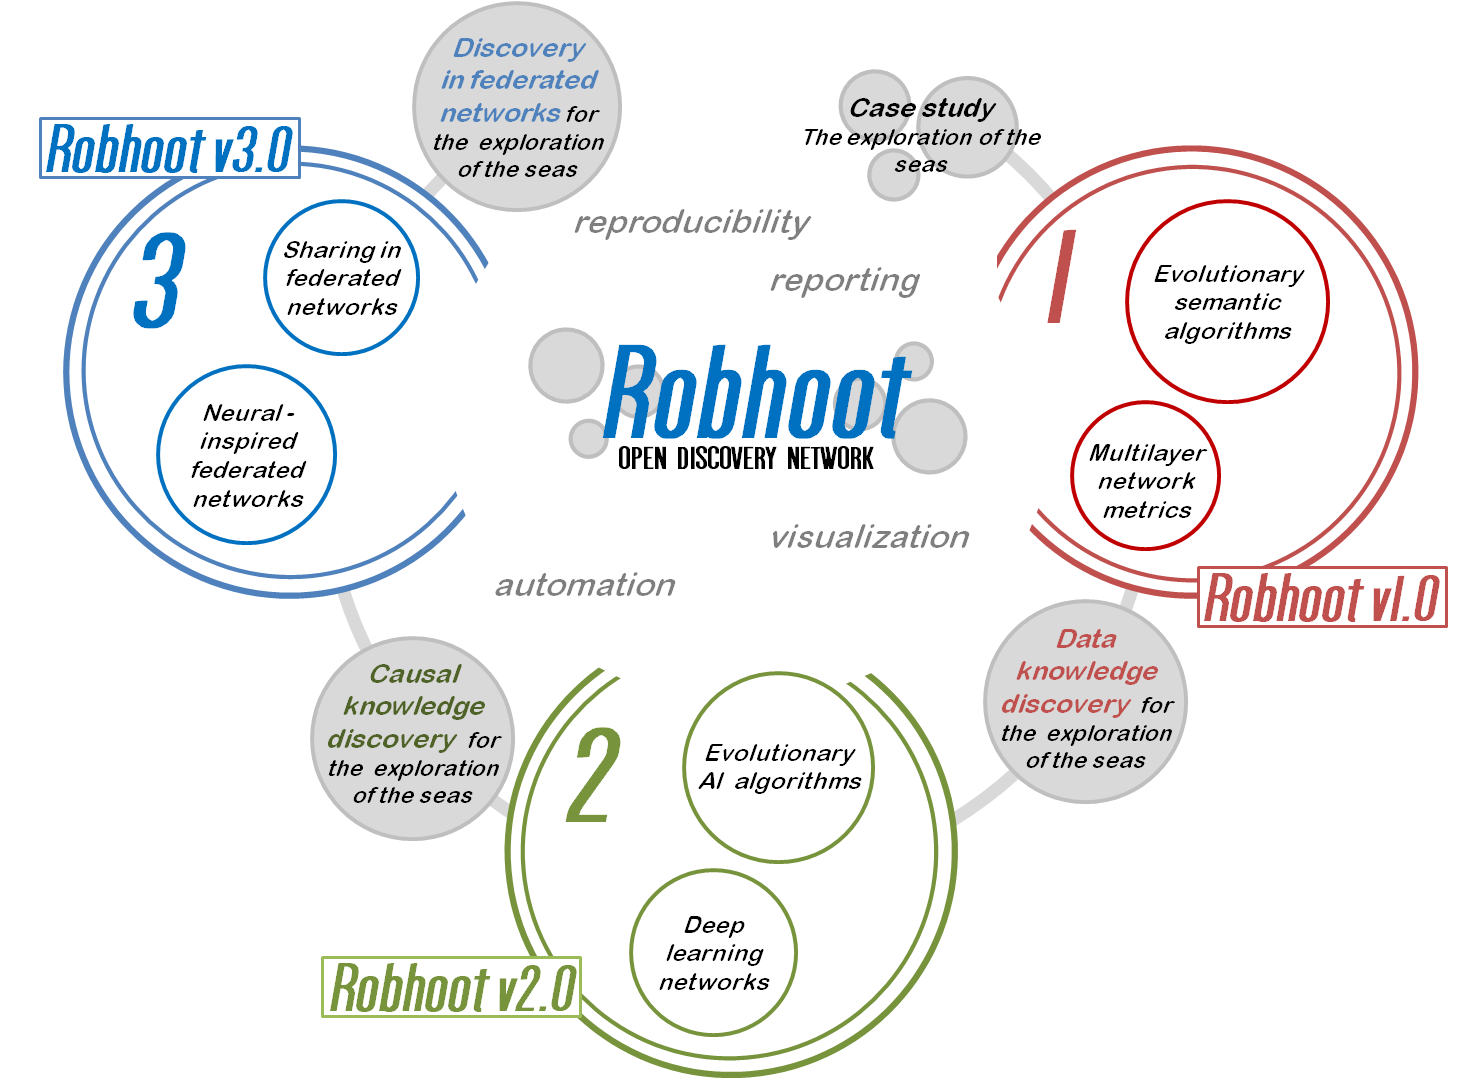
\includegraphics[width=16cm,height=12cm]{Figures/Robhoot_3f.png}
  \caption*{Figure 3: $\mathcal{ROBHOOT}$ delivers three work packages
    along three milestones: {\bf Data knowledge discovery} for the
    exploration of the seas in {\bf $\mathcal{ROBHOOT}$ v.1.0}. {\bf
      Causal knowledge discovery} for the exploration of the seas in
    {\bf $\mathcal{ROBHOOT}$ v.2.0}, and {\bf Discovery in Federated
      Networks} for the exploration of the seas integrating all
    features into one interdisciplinary science-enabled technology in
    {\bf $\mathcal{ROBHOOT}$ v.3.0}. Reproducibility, visualization,
    automation and reporting cross all the milestones to guarantee
    transparency and impact.}
   %Connect to Ghantt Chart (Table 3.1a), Work package (Table 3.1b)Acronyms of each deliverable and name lead: table 3.1c     
\end{figure}
  
  
  \subsection{Resources to be committed}
 
  \begin{itemize}
  \item \textcolor{red}{Please make sure the information in this
      section matches the costs as stated in the budget table in
      section 3 of the administrative proposal forms, and the number
      of person months, shown in the detailed work package
      descriptions.  Please provide the following:}
 \item \textcolor{red}{a table showing number of person months required
    (table 3.4a)}
  \item \textcolor{red}{a table showing ‘other direct costs’ (table
      3.4b) for participants where those costs exceed 15\% of the
      personnel costs (according to the budget table in section 3 of
      the administrative proposal forms)}
\end{itemize}

  

\newpage

\section{Members of the consortium}

\begin{comment}
 This section is not covered by the page limit.

 The information provided here will be used to judge the operational
 capacity. Please make sure that you do not include information here
 that relates to the headings under sections 1 to 3. Experts will be
 instructed to ignore any information here which appears to have been
 included to circumvent page limits applying to those sections.
 \end{comment}

 \subsection{Participants (applicants)}

 \begin{itemize}
 \item \textcolor{red}{For each participant, provide the following: a
     description of the legal entity and its main tasks, with an
     explanation of how its profile matches the tasks in the proposal}
 \item \textcolor{red}{a curriculum vitae or description of the
     profile of the persons, including their gender, who will be
     primarily responsible for carrying out the proposed research
     and/or innovation activities. Indicate each person who would be a
     first-time participant to FET under Horizon 2020}
\item \textcolor{red}{a list of up to 5 relevant publications, and/or
    products, services (including widely-used datasets or software),
    or other achievements relevant to the call content}
\item \textcolor{red}{List of up to 5 relevant previous projects or
    activities, connected to the subject of this proposal}
 \item \textcolor{red}{a description of any significant infrastructure
     and/or any major items of technical equipment, relevant to the
     proposed work}
 \item \textcolor{red}{if operational capacity cannot be demonstrated
     at the time of submitting the proposal, describe the concrete
     measures that will be taken to obtain it by the time of the
     implementation of the task}
 \end{itemize}


 \begin{itemize}
 \item (description legal identity) Dr. Carlos Meli\'an is a tenured
   researcher in Theoretical Evolutionary Ecology at EAWAG, ETH-Domain
   in Switzerland, and associate professor at the University of Bern.
       (CV, gender, responsible research proposed, first time participant FET)

       He is the principal coordinator of the proposal.  Dr. Meli\'an
       has broad expertise in evolutionary algorithms and
       eco-evolutionary dynamics in ecological communities and
       biodiversity.
  
       (5 pubs)
       • Melián C, et al. 2018. Deciphering the interdependence
       between ecological and evolutionary networks. Trends in ecology
       & evolution 33,7: 504-512.  • Andreazzi C, Guimaraes P, Melián
       C. 2018. Eco-evolutionary feedbacks promote fluctuating
       selection and long-term stability of antagonistic
       networks. Proc. R. Soc. B 285: 20172596.  • Melián C, Seehausen
       O, Eguiluz V, Fortuna M, Deiner K. 2015. Diversification and
       Biodiversity Dynamics of Hot and Cold Spots. Ecography 38,
       393-401.  • Melián C, et al. 2015. Dispersal dynamics in food
       webs. American Naturalist 185, 2: 157-168.  • Melián C., et
       al. 2014. Individual trait variation and diversity in food
       webs. Advances in Ecological Research. Vol. 50. Academic Press,
       207-241.



 \item {\bf Victor M. Egu\'iluz (IFISC, CSIC, Spain)}: IFISC is an
   Maria de Maetzu Excellent center at the UIB, Balearic
   Islands. Dr. Egu\'iluz has expertise in health-related topics, in
   particular he has developed collaborations with Harvard medical
   school and many biodiversity and sustainability research
   institutions. The group of the PL has worked in the development of
   data-driven agent-based networks in social, biological and
   environmental problems with particular relevance in epidemiological
   networks.
\item
\item
   \end{itemize}

 
 \subsection{Third parties involved in the project (including use of third party resources)}


\begin{itemize}
\item \textcolor{red}{For each participant, does the participant plan
    to subcontract certain tasks (please note that core tasks of the
    project should not be sub-contracted) Y/N If yes, please describe
    and justify the tasks to be subcontracted}
\item \textcolor{red}{Does the participant envisage that part of its
    work is performed by linked third parties2 Y/N If yes, please
    describe the third party, the link of the participant to the third
    party, and describe and justify the foreseen tasks to be performed
    by the third party}
\item \textcolor{red}{Does the participant envisage the use of
    contributions in kind provided by third parties (Articles 11 and
    12 of the General Model Grant Agreement) Y/N If yes, please
    describe the third party and their contributions}
\item \textcolor{red}{Does the participant envisage that part of the
    work is performed by International Partners3 (Article 14a of the
    General Model Grant Agreement)?  Y/N If yes, please describe the
    International Partner(s) and their contributions.}
\end{itemize}


\section{Ethics and Security}

 This section is not covered by the page limit.

\subsection{Ethics}


\textcolor{red}{ For more guidance, see the document "How to complete
  your ethics self-assessment".  If you have entered any ethics issues
  in the ethical issue table in the administrative proposal forms, you
  must:}

\begin{itemize}
\item \textcolor{red}{submit an ethics self-assessment, which:}
\item \textcolor{red}{describes how the proposal meets the national
    legal and ethical requirements of the country or countries where
    the tasks raising ethical issues are to be carried out;}
\item \textcolor{red}{explains in detail how you intend to address the
    issues in the ethical issues table, in particular as regards:
    research objectives (e.g. study of vulnerable populations, dual
    use, etc.)  ▪ research methodology (e.g. clinical trials,
    involvement of children and related consent procedures, protection
    of any data collected, etc.)}
\item \textcolor{red}{the potential impact of the research (e.g. dual
    use issues, environmental damage, stigmatisation of particular
    social groups, political or financial retaliation,
    benefit-sharing, misuse, etc.)}
\item \textcolor{red}{provide the documents that you need under
    national law(if you already have them), e.g.: ◦ an ethics
    committee opinion; ◦ the document notifying activities raising
    ethical issues or authorising such activities If these documents
    are not in English, you must also submit an English summary of
    them (containing, if available, the conclusions of the committee
    or authority concerned).

    \\
    If you plan to request these documents specifically for the project
  you are proposing, your request must contain an explicit reference
  to the project title.}

\subsection{Security}


\textcolor{red{Please indicate if your project will involve:}

\begin{itemize}
\item \textcolor{red}{activities or results raising security issues:
    (YES/NO)}
\item \textcolor{red}{EU-classified information as background or
    results: (YES/NO)}
\end{itemize}  



%----------------------------------------------------------------------------------------
%	BIBLIOGRAPHY
%----------------------------------------------------------------------------------------

%\printbibliography[title={Bibliography}] % Print the bibliography, section title in curly brackets

\newpage
\bibliographystyle{unsrtnat}
%\bibliographystyle{tree.bst}
\bibliography{Robhoot.bib}

%----------------------------------------------------------------------------------------

\end{document}
